% Copyright 2004 by Till Tantau <tantau@users.sourceforge.net>.
%
% In principle, this file can be redistributed and/or modified under
% the terms of the GNU Public License, version 2.
%
% However, this file is supposed to be a template to be modified
% for your own needs. For this reason, if you use this file as a
% template and not specifically distribute it as part of a another
% package/program, I grant the extra permission to freely copy and
% modify this file as you see fit and even to delete this copyright
% notice. 

\documentclass{beamer}

% There are many different themes available for Beamer. A comprehensive
% list with examples is given here:
% http://deic.uab.es/~iblanes/beamer_gallery/index_by_theme.html
% You can uncomment the themes below if you would like to use a different
% one:
%\usetheme{AnnArbor}
%\usetheme{Antibes}
%\usetheme{Bergen}
%\usetheme{Berkeley}
%\usetheme{Berlin}
%\usetheme{Boadilla}
%\usetheme{boxes}
%\usetheme{CambridgeUS}
%\usetheme{Copenhagen}
%\usetheme{Darmstadt}
%\usetheme{default}
%\usetheme{Frankfurt}
%\usetheme{Goettingen}
%\usetheme{Hannover}
%\usetheme{Ilmenau}
%\usetheme{JuanLesPins}
%\usetheme{Luebeck}
%\usetheme{Madrid}
%\usetheme{Malmoe}
%\usetheme{Marburg}
%\usetheme{Montpellier}
%\usetheme{PaloAlto}
%\usetheme{Pittsburgh}
%\usetheme{Rochester}
%\usetheme{Singapore}
%\usetheme{Szeged}
%\usetheme{Warsaw}

\usepackage{amsmath}
\usepackage{textpos}
\usepackage{ulem}

\definecolor{BYUblue}{RGB}{0,31,69}
\definecolor{BYUgold}{RGB}{195,163,106}
\usecolortheme[RGB={0,31,69}]{structure} % BYU Blue

\definecolor{metric-PR}{RGB}{200,127,0}
\definecolor{metric-NE}{RGB}{51,51,255}
\definecolor{metric-OFI}{RGB}{204,0,0}
\definecolor{metric-IRO}{RGB}{0,102,51}

\usetheme{Frankfurt}
\setbeamercolor*{section in head/foot}{bg=BYUblue,fg=gray!25}
\setbeamercolor*{frametitle}{bg=BYUblue!50,fg=white!25}
\setbeamercovered{transparent}
\mode<all>

\DeclareMathOperator*{\argmax}{arg\,max}

\title{Submodular optimization}

%\subtitle{Optional Subtitle}

\author{ Daqing Yi }


\institute
{
  HCMI lab\\
  Brigham Young University
}

\date[]{} 

\addtobeamertemplate{frametitle}{}
{
\begin{textblock*}{100mm}(0.9\textwidth,-1.2cm)

\includegraphics[width=1.1cm]{figure/BYU_logo.png}
\end{textblock*}
}

\begin{document}

\begin{frame}
  \titlepage
\end{frame}

\begin{frame}{Outline}{Structure}
  \tableofcontents
  % You might wish to add the option [pausesections]
\end{frame}

\section{Introduction}

\begin{frame}{Modeling human intent}{Path Planning}
THe problem in modeling human intent
\begin{itemize}
\item incomparability in objectives
\item conflict in objectives
\item hardness in weighing the objectives
\item vagueness in importance selection
\end{itemize}
\begin{figure}
\centering
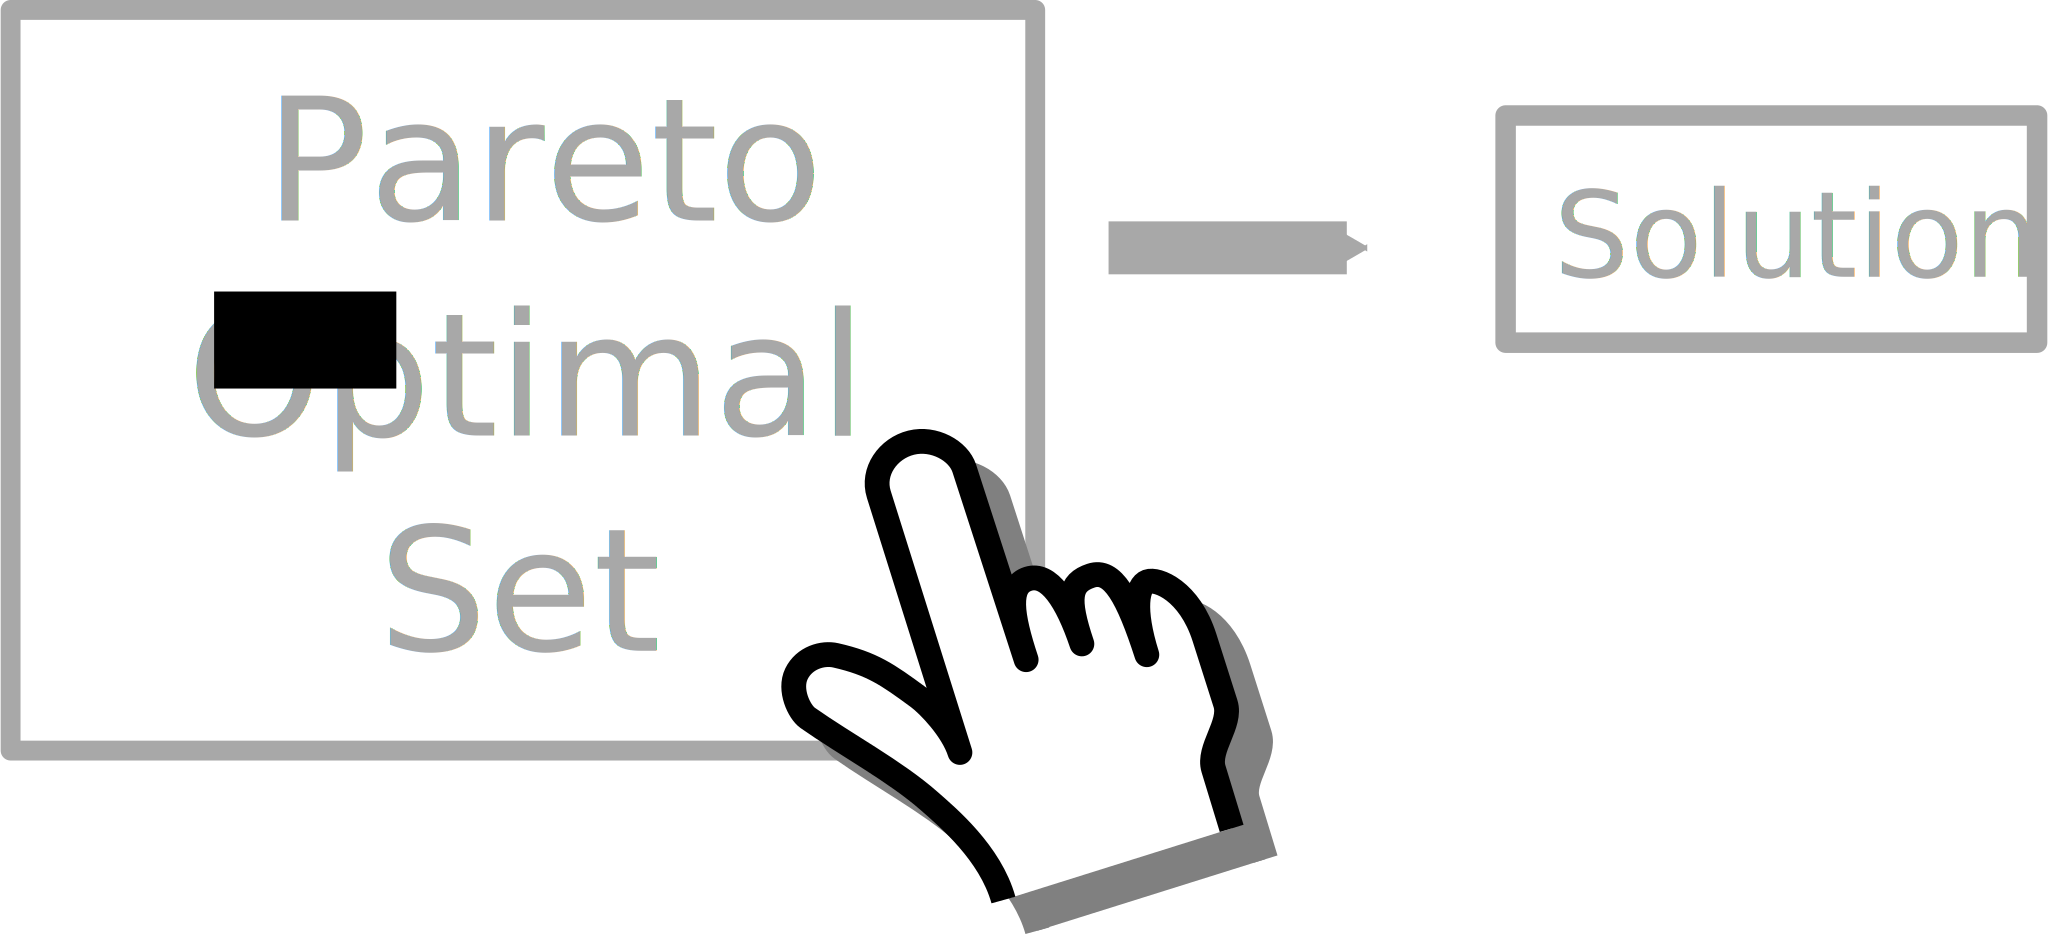
\includegraphics[width=0.6\linewidth]{figure/human_interactive_moo}
%\caption{}
\label{fig:human_interactive_moo}
\end{figure}
\end{frame}

\begin{frame}{Pareto Optimal}{}
\end{frame}

\section{Submodular}

\begin{frame}{Submodular}{Submodular}
\begin{frame}
	\begin{block}{}
		\begin{equation}
		\nonumber
		f(x_{1} , \cdots , x_{N} )= f(x_{1}) + \cdots + f(x_{N})
		\end{equation}
	\end{block}
\end{frame}
\end{frame}

\begin{frame}{Sensor placement}{Maximum coverage}
	
\end{frame}

\begin{frame}{Sensor placement}{MAP inference}
	
\end{frame}


\section{Path Planning}

\begin{frame}{Informative Path Planning}{Information measurement}
\begin{itemize}
\item minimize the uncertainty of the observed environment
\end{itemize}
\begin{figure}
	\centering
	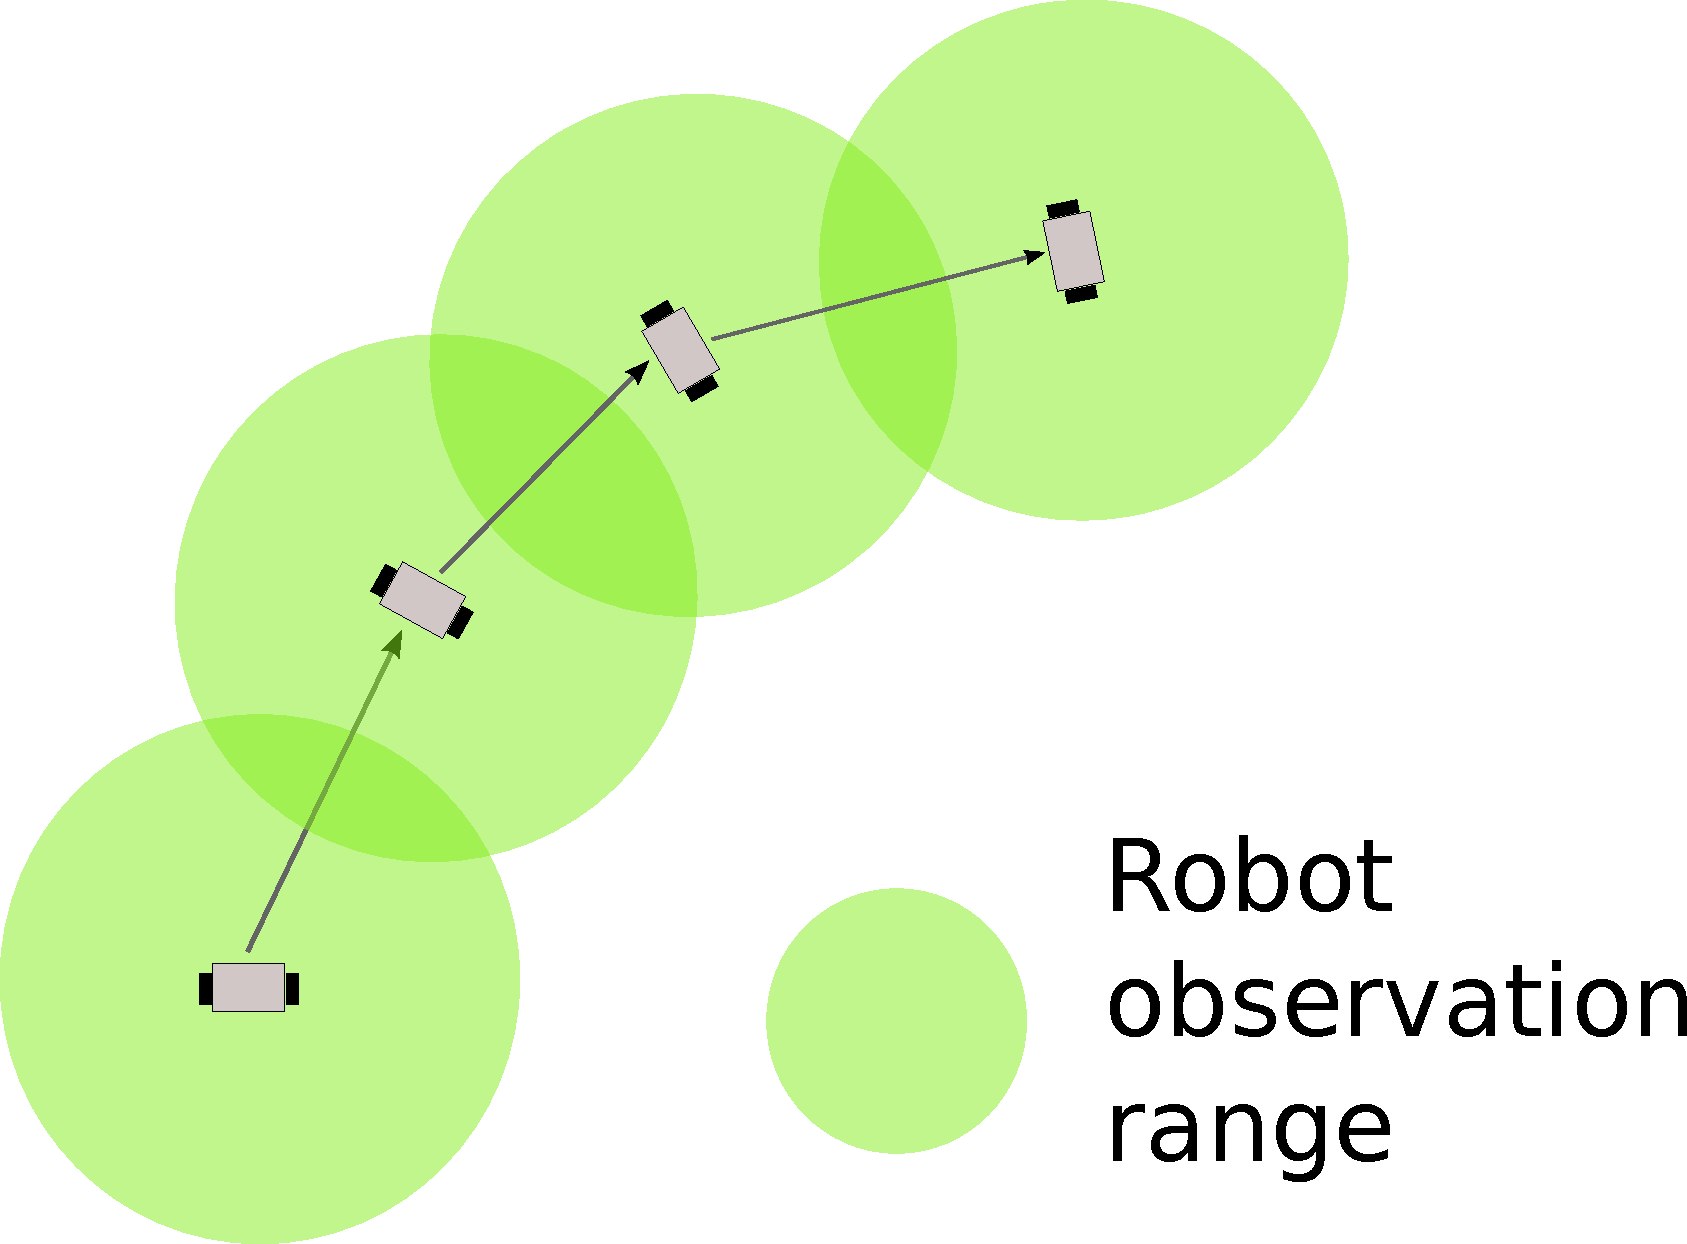
\includegraphics[width = .6\textwidth]{./figure/robotObservation}
\end{figure}
\end{frame}

\begin{frame}{Cordon and search}{Application}
\begin{columns}
	\column{0.5\textwidth}
	\begin{minipage}{\textwidth}
		\begin{figure}
			\centering
			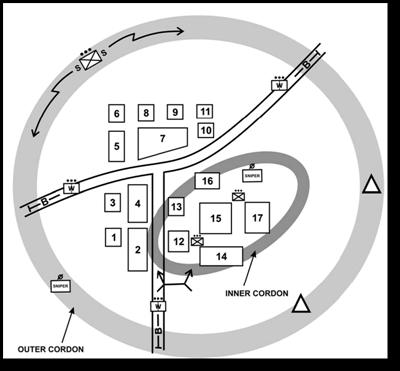
\includegraphics[width = 0.9\textwidth]{./figure/cordon_and_search.jpg}
		\end{figure}
	\end{minipage}
	
	\column{0.5\textwidth}
	\begin{minipage}{\textwidth}
		\begin{figure}
			\centering
			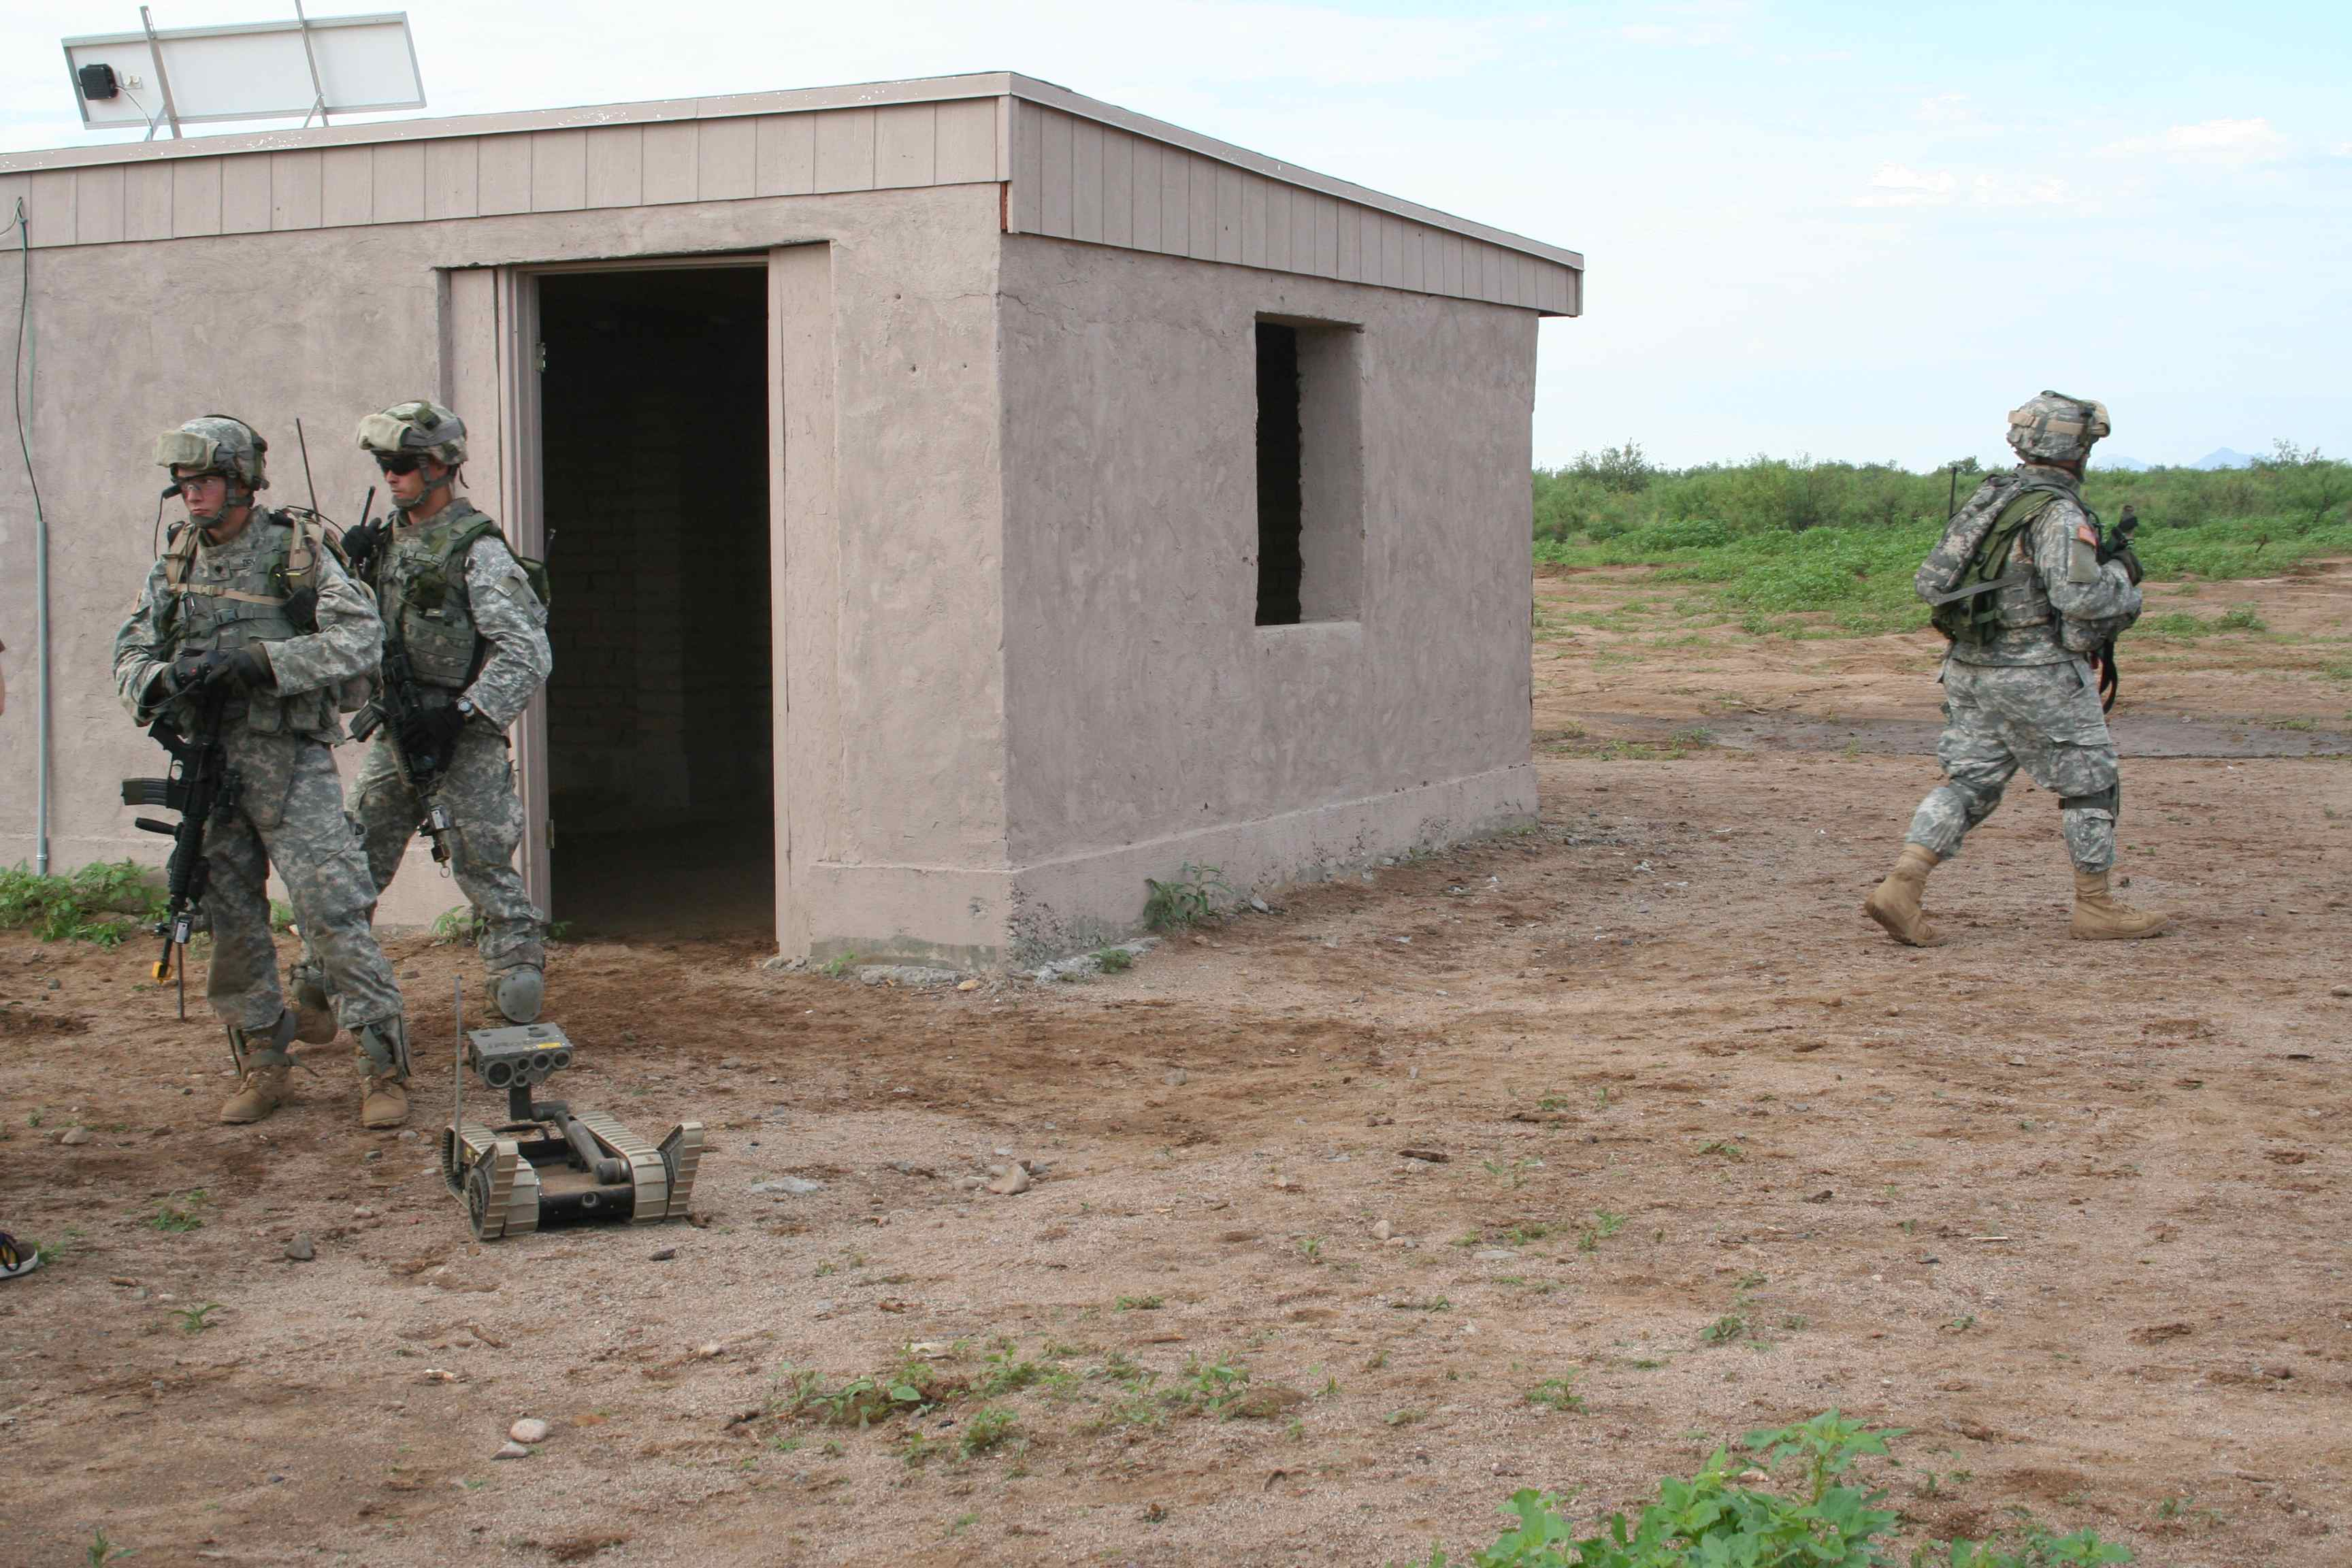
\includegraphics[width = 0.9\textwidth]{./figure/soldier_and_robot.jpg}
		\end{figure}
	\end{minipage}	
\end{columns}
\end{frame}

\begin{frame}{Map discretization}{Application}
	\begin{columns}
		\column{0.5\textwidth}
		\begin{minipage}{\textwidth}
			\begin{figure}
				\centering
				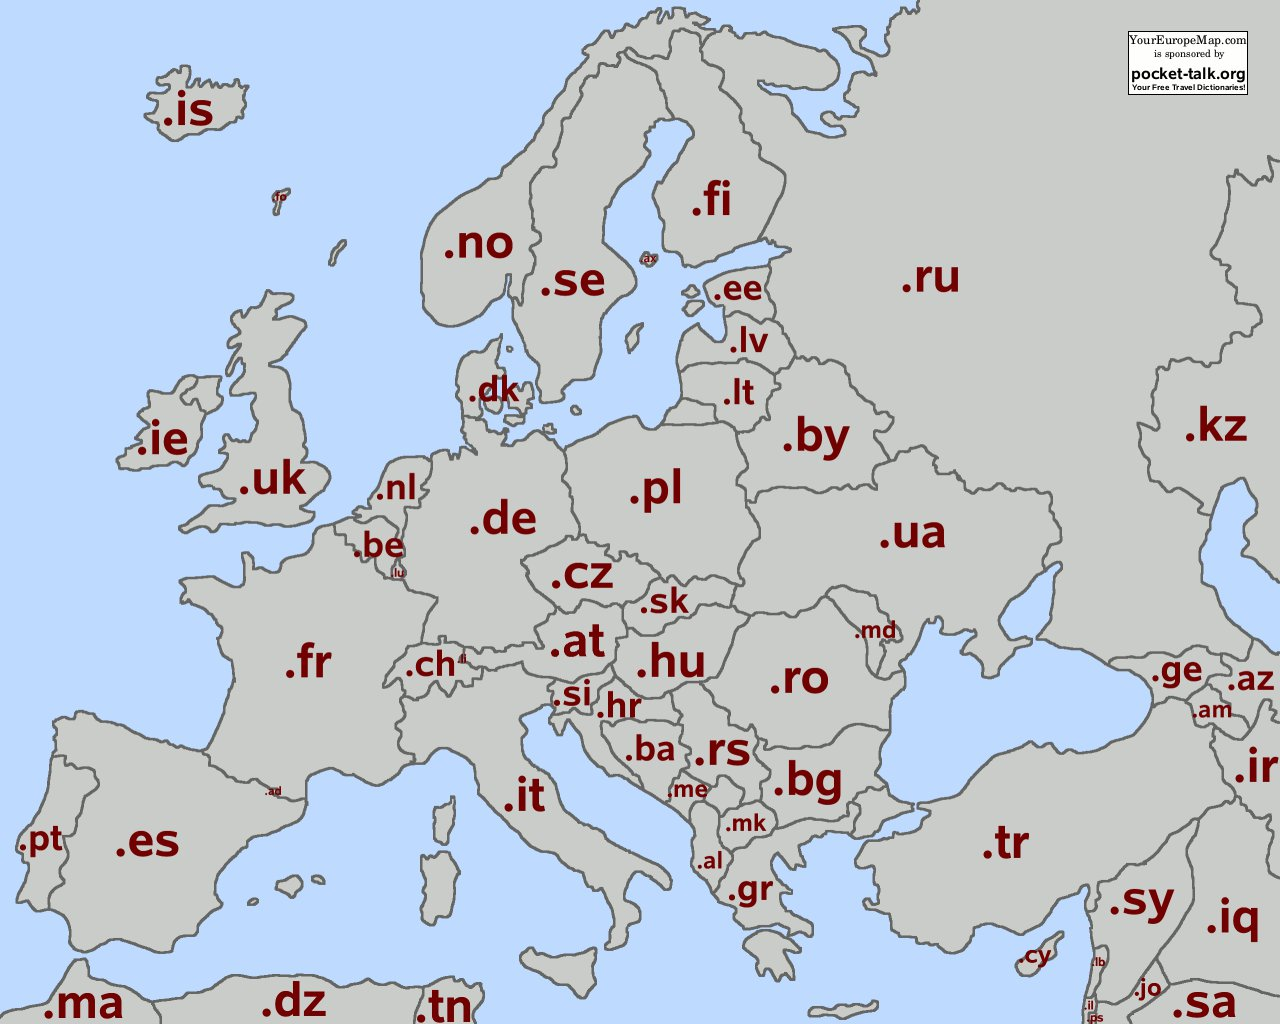
\includegraphics[width = 0.9\textwidth]{./figure/map_tld_europe.jpg}
			\end{figure}
		\end{minipage}
		
		\column{0.5\textwidth}
		\begin{minipage}{\textwidth}
			\begin{figure}
				\centering
				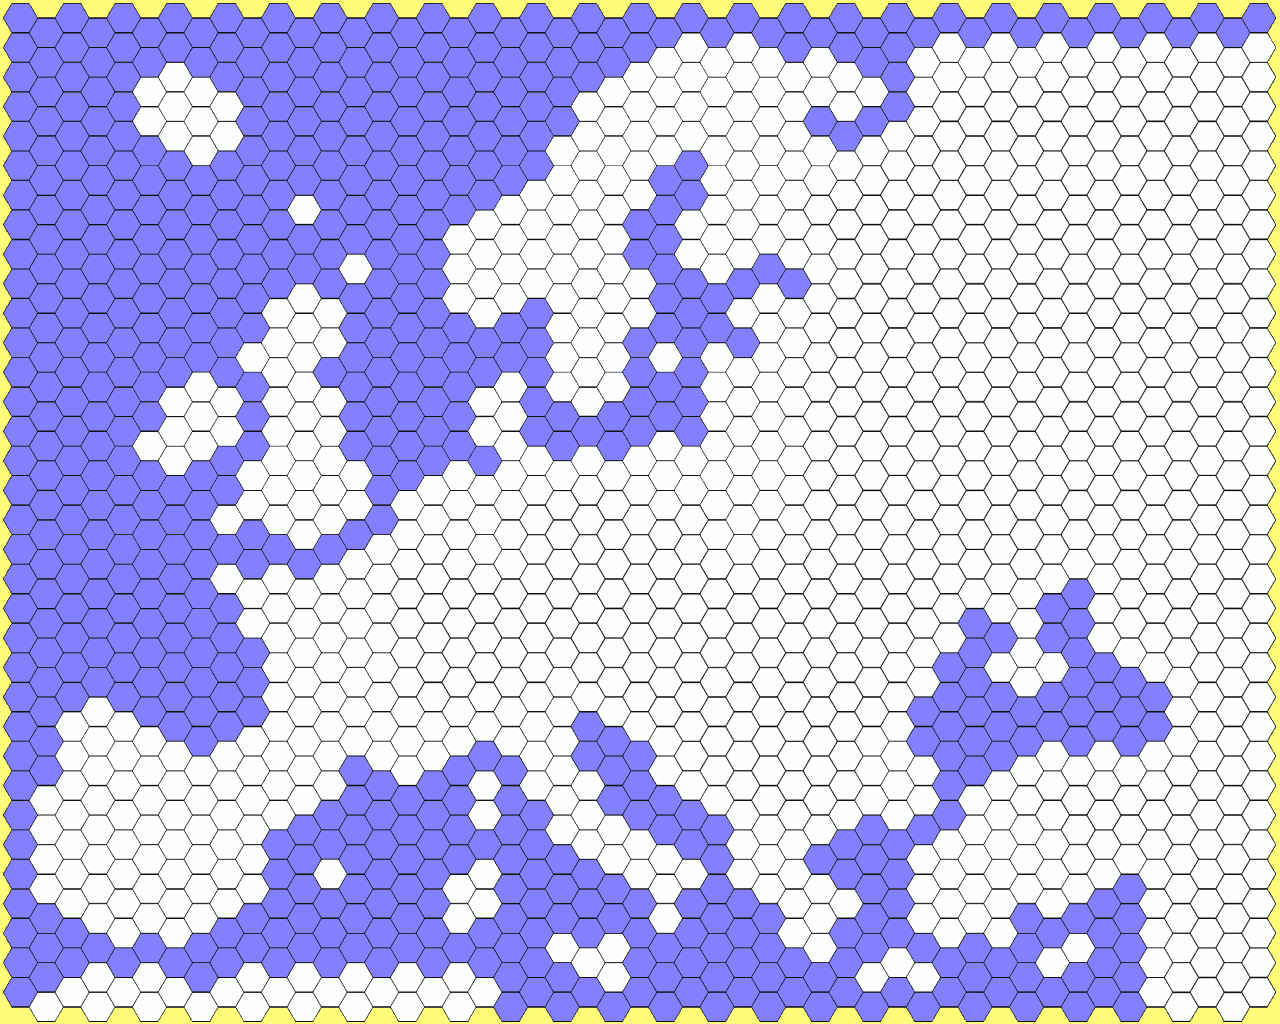
\includegraphics[width = 0.9\textwidth]{./figure/hexagonal_europe_map.png}
			\end{figure}
		\end{minipage}	
	\end{columns}
\end{frame}

\begin{frame}{Submodular orienteering}{Informative path}
	\begin{itemize}
	\item $ \mathbf{S} $ - Environment states
	\item $ \mathbf{O}^{X} $ - Robot's observations
	\item $ \mathbf{O}^{Y^{h}} $ - Human's obeservations
	\end{itemize}
	\begin{block}{Conditional mutual information}
		$ I(\mathbf{S}; \mathbf{O}^{X} \mid \mathbf{O}^{Y^{h}}) = H(\mathbf{S} \mid \mathbf{O}^{Y^{h}}) - H(\mathbf{S} \mid \mathbf{O}^{X},\mathbf{O}^{Y^{h}}) $
	\end{block} 
	
	\bigskip
	
	\begin{itemize}
		\item Entropy reduction
		\item Submodularity
		\item Chain rule \\
		$ I(\mathbf{S}; \mathbf{O}^{X} \mid \mathbf{O}^{Y^{h}}) = \sum_{t=1}^{T} I(O^{X}_{t} ; \mathbf{S} \mid O^{X}_{1} , \cdots , O^{X}_{t-1}, \mathbf{O}^{Y^{h}}) $
	\end{itemize}
	
\end{frame}

%\subsection{Human constraint}

\begin{frame}{Team role}{Human constraint}
	
	\begin{figure}
		\centering
		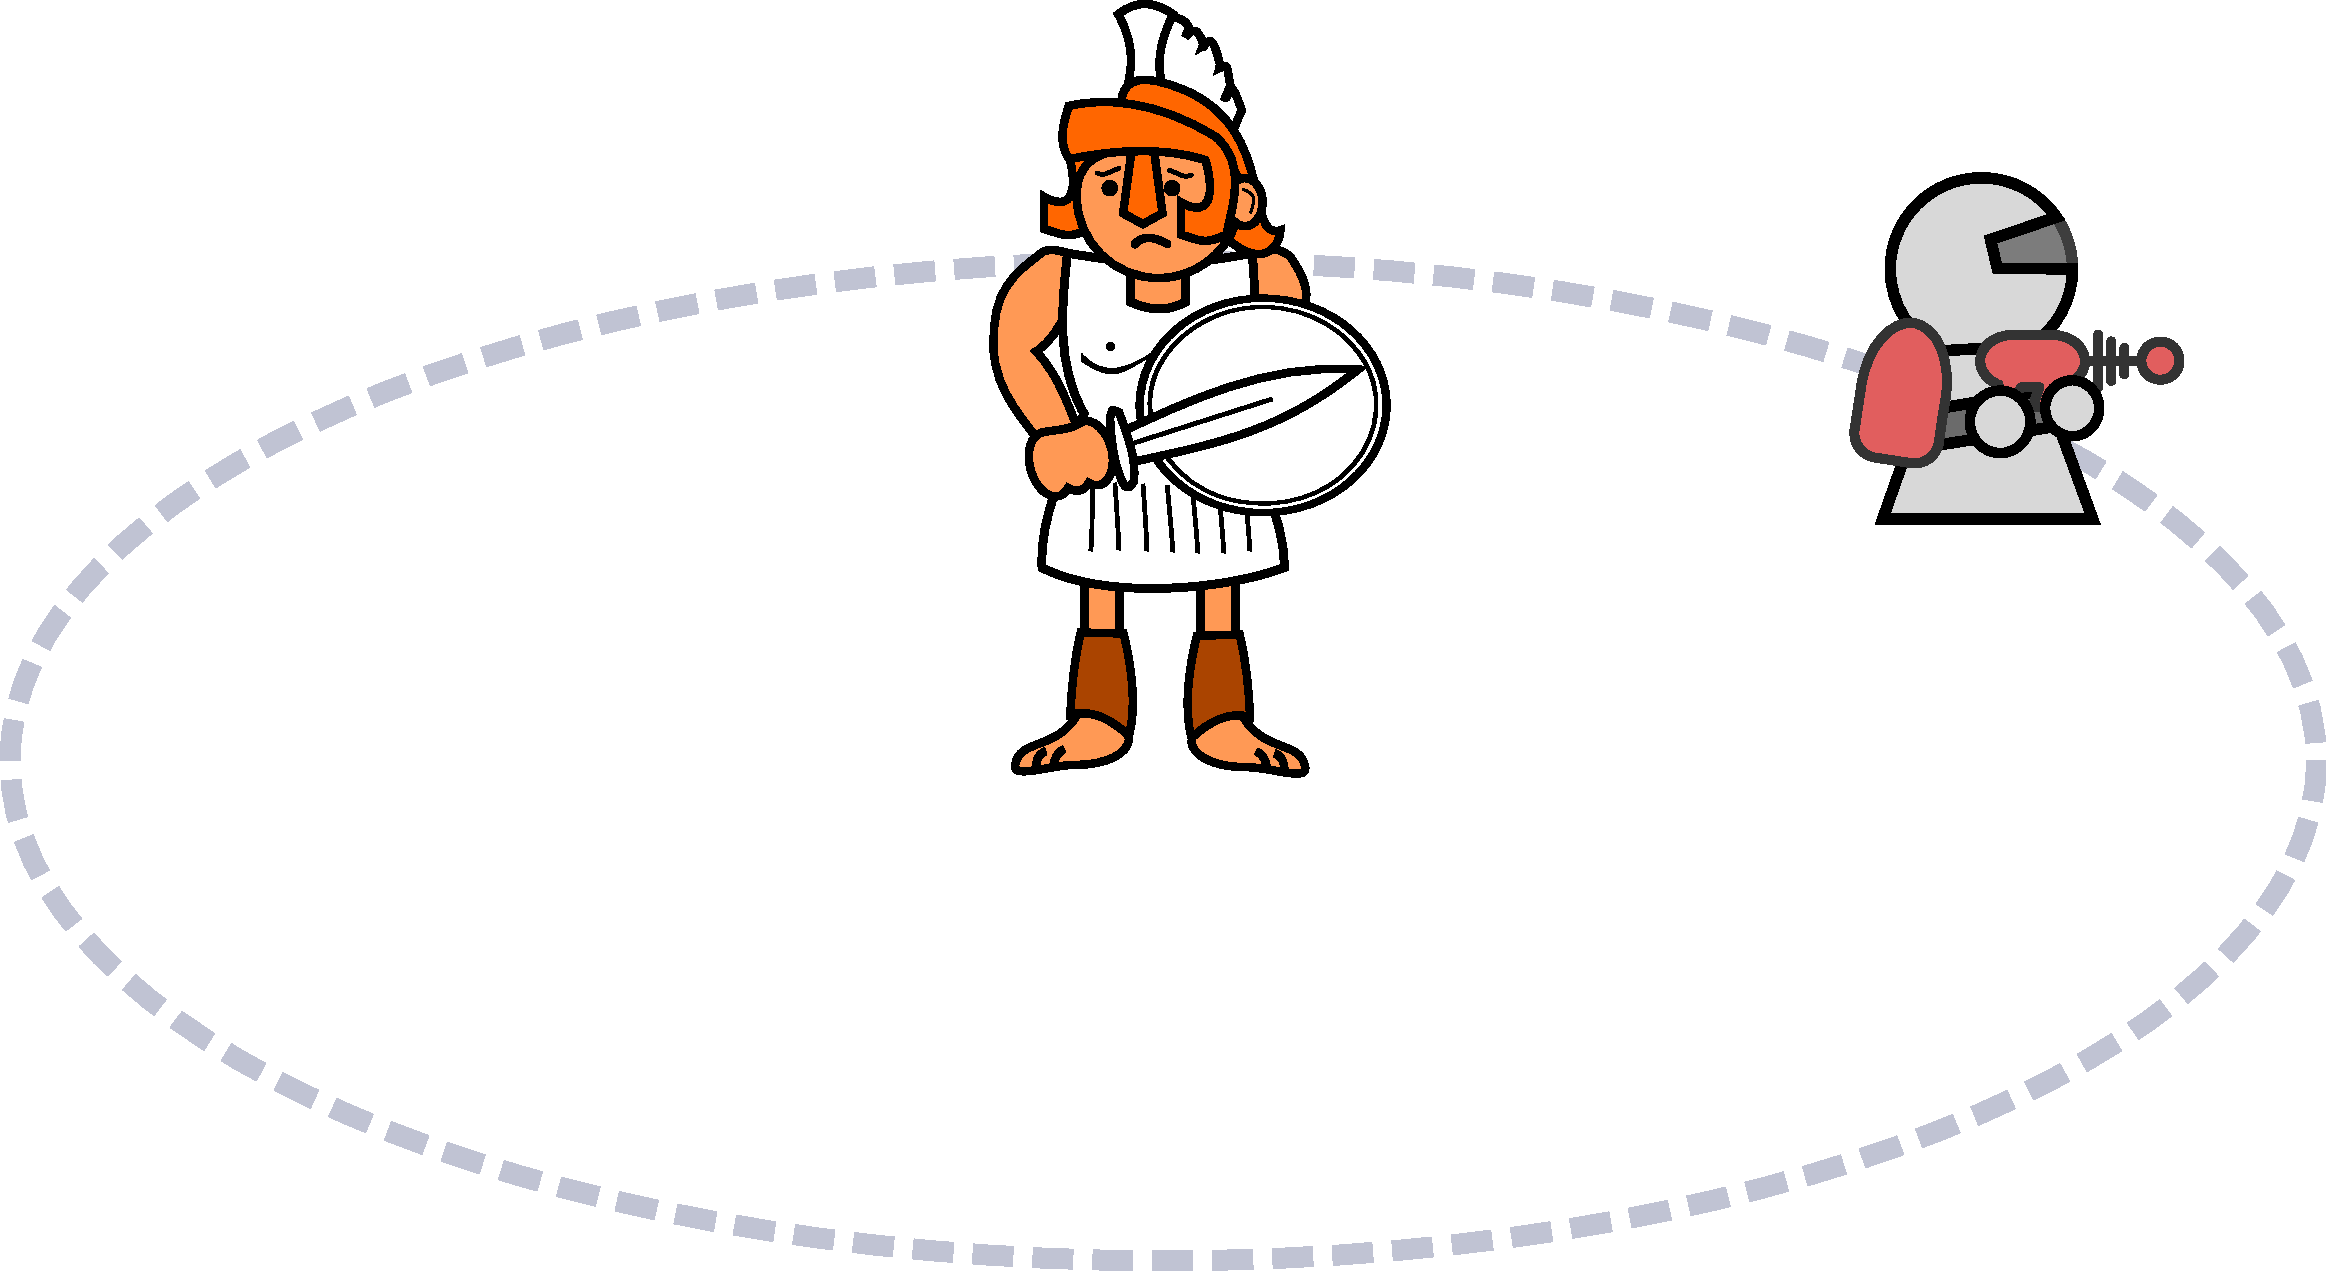
\includegraphics[width = 0.7\textwidth]{./figure/human_robot_interaction}
	\end{figure}
	
	\begin{itemize}
		\item cooperative observation
		\item assistance and protection
	\end{itemize}
	
\end{frame}

\begin{frame}{Neighboring function}{Human constraint}
	\begin{columns}
		\column{.6\linewidth}
		\begin{minipage}[c]{\linewidth}
			\begin{figure}
				\centering
				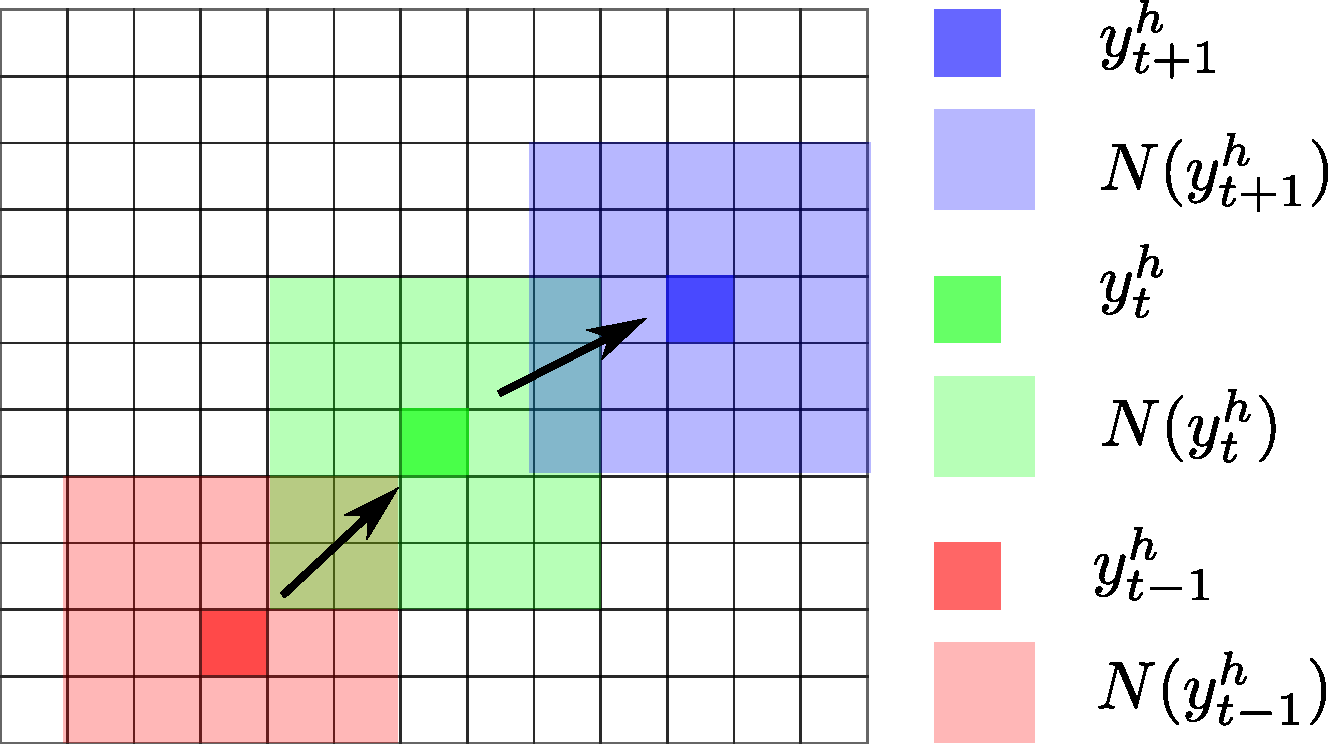
\includegraphics[width = \textwidth]{./figure/humanConstraint}
				%\caption{An example of human constraint.}
			\end{figure}
		\end{minipage}
		
		\column{.4\linewidth}
		\begin{minipage}[c]{\linewidth}
			\begin{itemize}
				\item { human path $ \{ y^{h}_{1} \cdots y^{h}_{T} \} $ }
				\item { neighboring function $ N( y^{h}_{t} ) $ }
			\end{itemize}
		\end{minipage}
	\end{columns}
	
\end{frame}

\begin{frame}{Related work}{ Using a greedy heuristic}
\begin{block}{C.~Chekuri 2005\cite{1530718}}
\begin{itemize}
\item Recursive greedy on a graph topoplogy
\item Edge cost $ \Rightarrow $ Budget 
\end{itemize}
\end{block}
\begin{block}{A.~Singh 2007\cite{singh2007efficient}}
\begin{itemize}
\item Spatial decomposition
\item Recursive greedy of multiple robots
\end{itemize}
\end{block}
\end{frame}

\begin{frame}{Related work}{Using a coarse-to-fine dynamic programming}
\begin{block}{C.~Raphael 2001\cite{Raphael2001}}
Coarse-to-fine backtracking
\end{block}
\begin{figure}
	\centering
	\includegraphics[width = 0.5\textwidth]{./figure/coarse_to_fine_DP}
\end{figure}
\end{frame}






\section{Human constraint}

\begin{frame}{Human constraint}{constraint}

\end{frame}

\section{Problem definition}

\subsection{Informative path}

\begin{frame}{Coverage model}{Informative path}

\begin{itemize}
\item Information measurement - entropy 
\item Maximum coverage problem
\end{itemize}

\begin{figure}
\centering
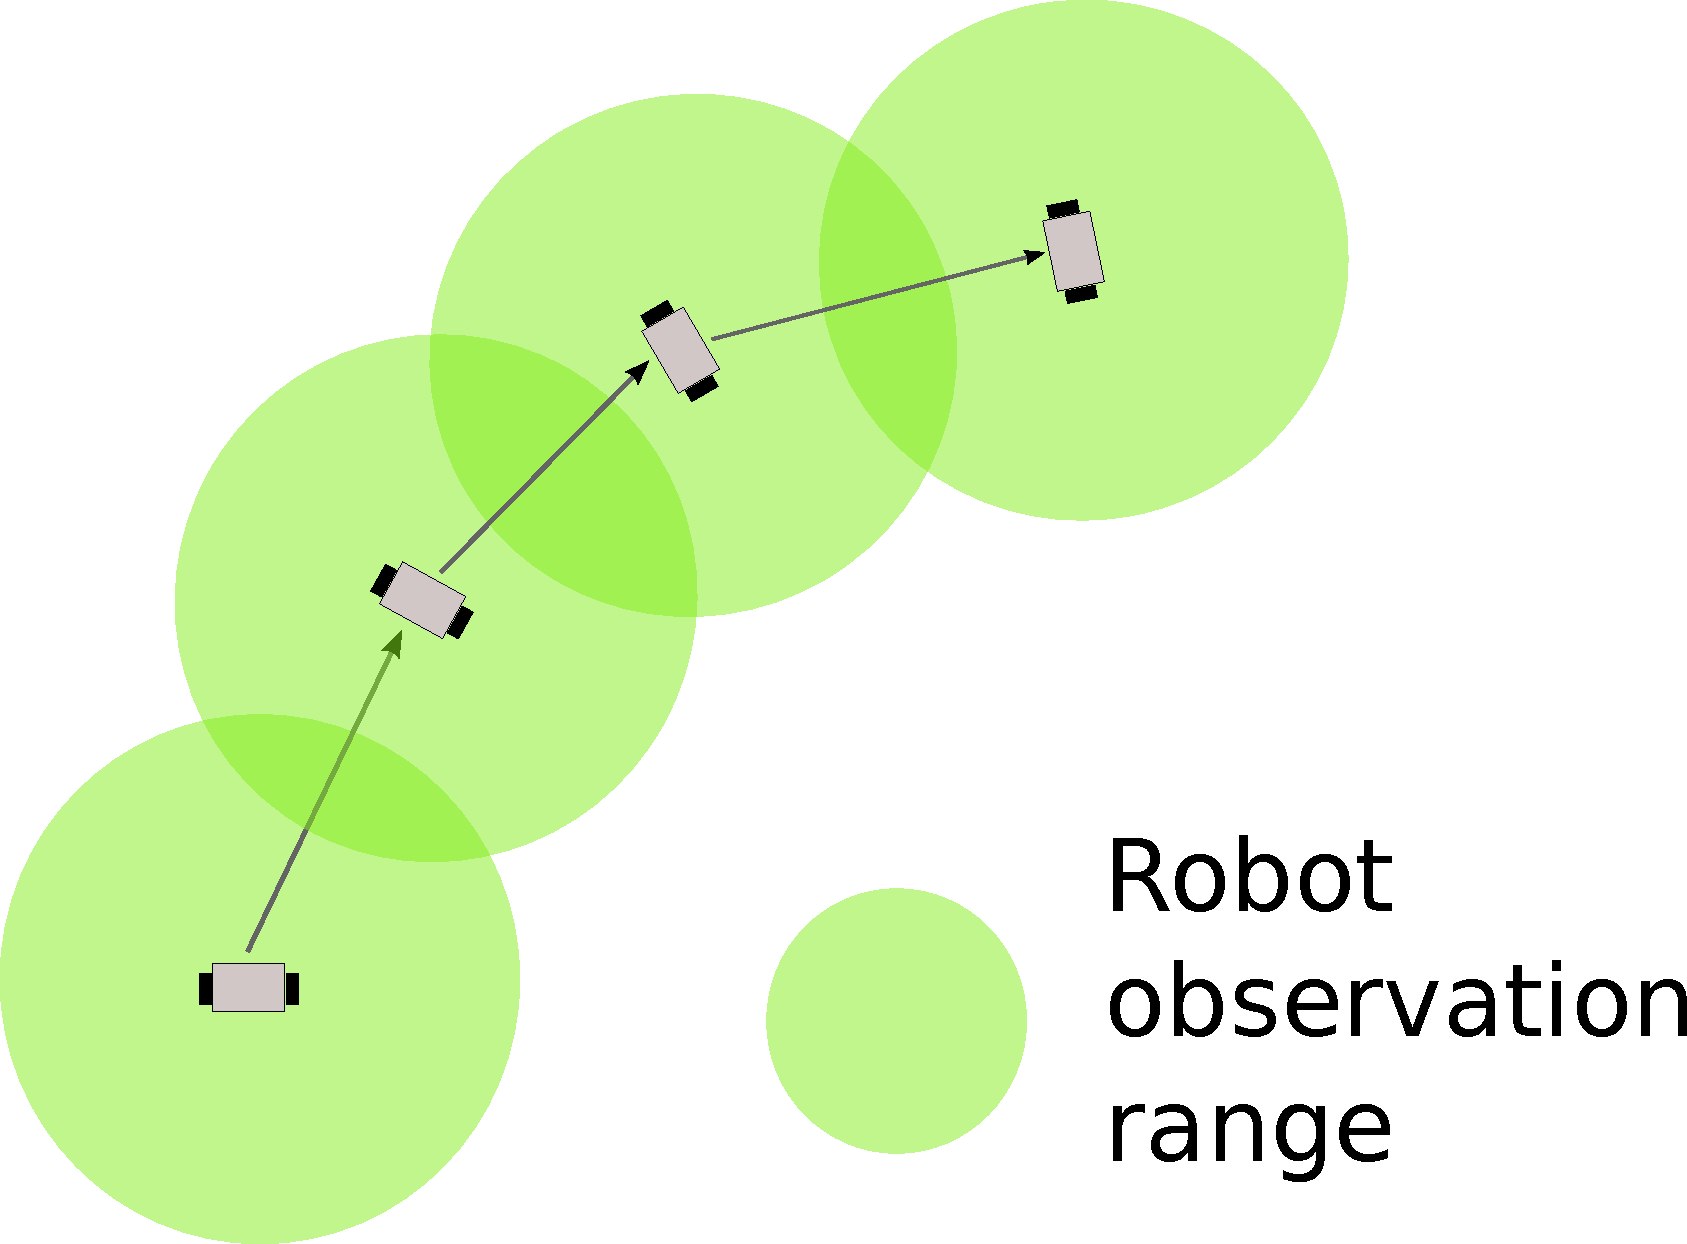
\includegraphics[width = 0.6\textwidth]{./figure/robotObservation}
%\caption{A coverage model.}
\end{figure}

\end{frame}

\begin{frame}{Submodularity}{Informative path}

\begin{columns}

\column{0.45\textwidth}

\begin{figure}
\centering
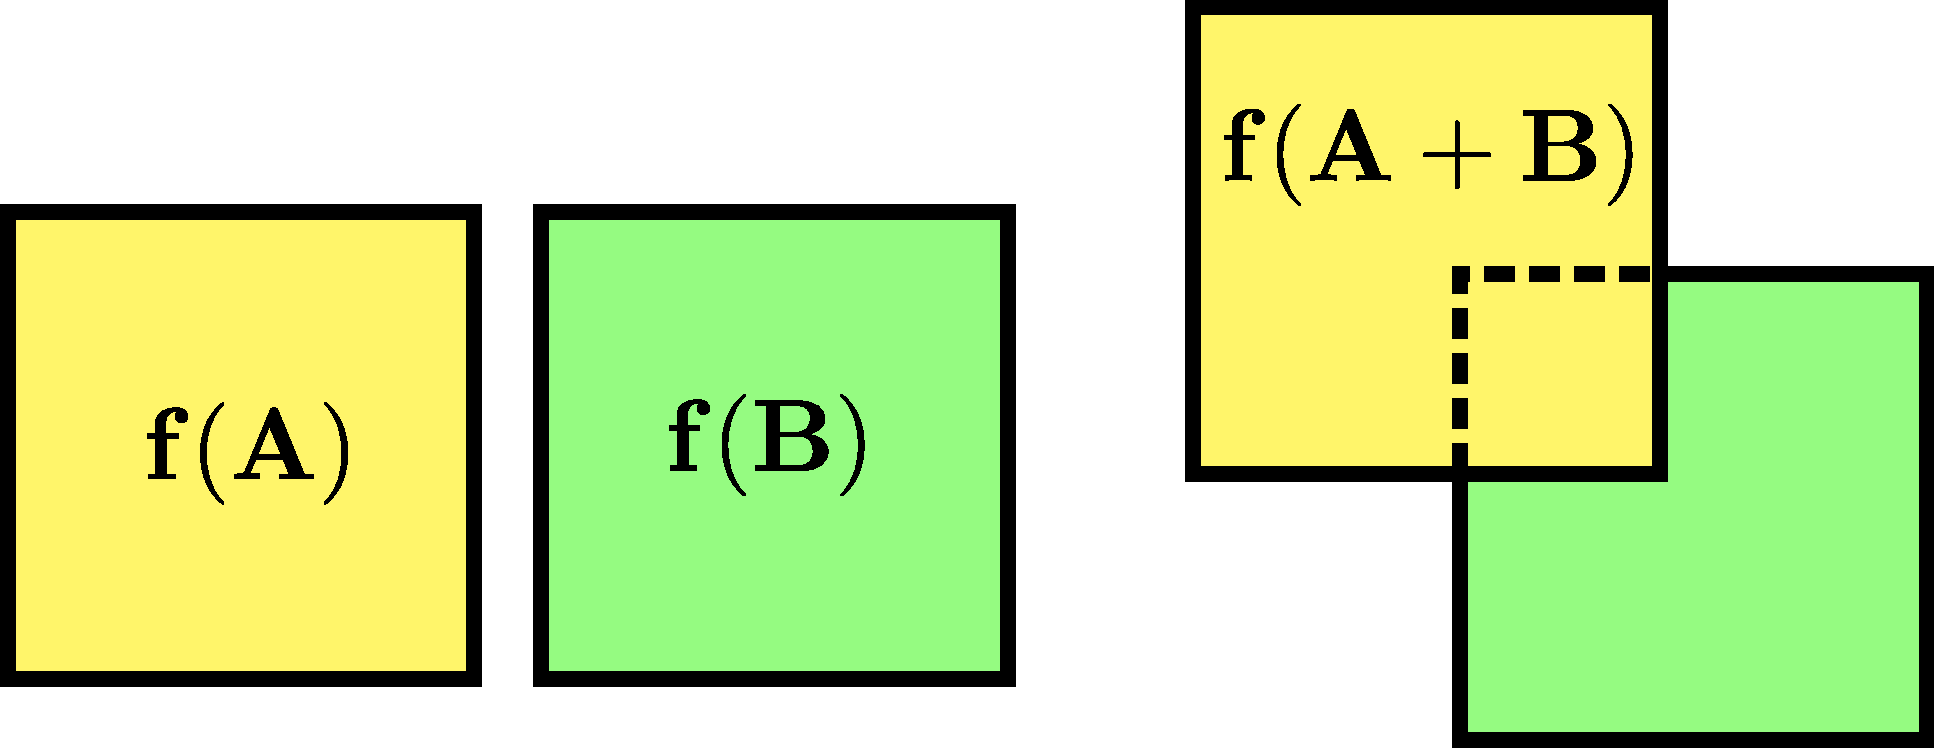
\includegraphics[width = \textwidth]{./figure/submodular}
%\caption{A coverage model.}
\end{figure}

\begin{equation}
\nonumber
f(A) + f(B) \geq f(A+B)
\end{equation}

\column{0.1\textwidth}

\column{0.45\textwidth}

Information
\begin{itemize}
\item search space $ S $
\item the observation of a robot $ \mathbf{O}^{X} $ 
\item the observation of a human $ \mathbf{O}^{Y} $

\bigskip
\bigskip

$ f( \mathbf{S}, \mathbf{O}^{X} ) + f( \mathbf{S}, \mathbf{O}^{Y^{h}} ) \geq f( \mathbf{S}, \mathbf{O}^{X},  \mathbf{O}^{Y^{h}} ) $ 
\end{itemize}

\end{columns}

\end{frame}

\begin{frame}{Submodular orienteering}{Informative path}

\begin{block}{Conditional mutual information}
$ I(\mathbf{S}; \mathbf{O}^{X} \mid \mathbf{O}^{Y^{h}}) = H(\mathbf{S} \mid \mathbf{O}^{Y^{h}}) - H(\mathbf{S} \mid \mathbf{O}^{X},\mathbf{O}^{Y^{h}}) $
\end{block} 

\bigskip

\begin{itemize}
\item Entropy reduction
\item Submodularity
\item Chain rule \\
$ I(\mathbf{S}; \mathbf{O}^{X} \mid \mathbf{O}^{Y^{h}}) = \sum_{t=1}^{T} I(O^{X}_{t} ; \mathbf{S} \mid O^{X}_{1} , \cdots , O^{X}_{t-1}, \mathbf{O}^{Y^{h}}) $
\end{itemize}

\end{frame}

\subsection{Human constraint}

\begin{frame}{Team role}{Human constraint}

\begin{figure}
\centering
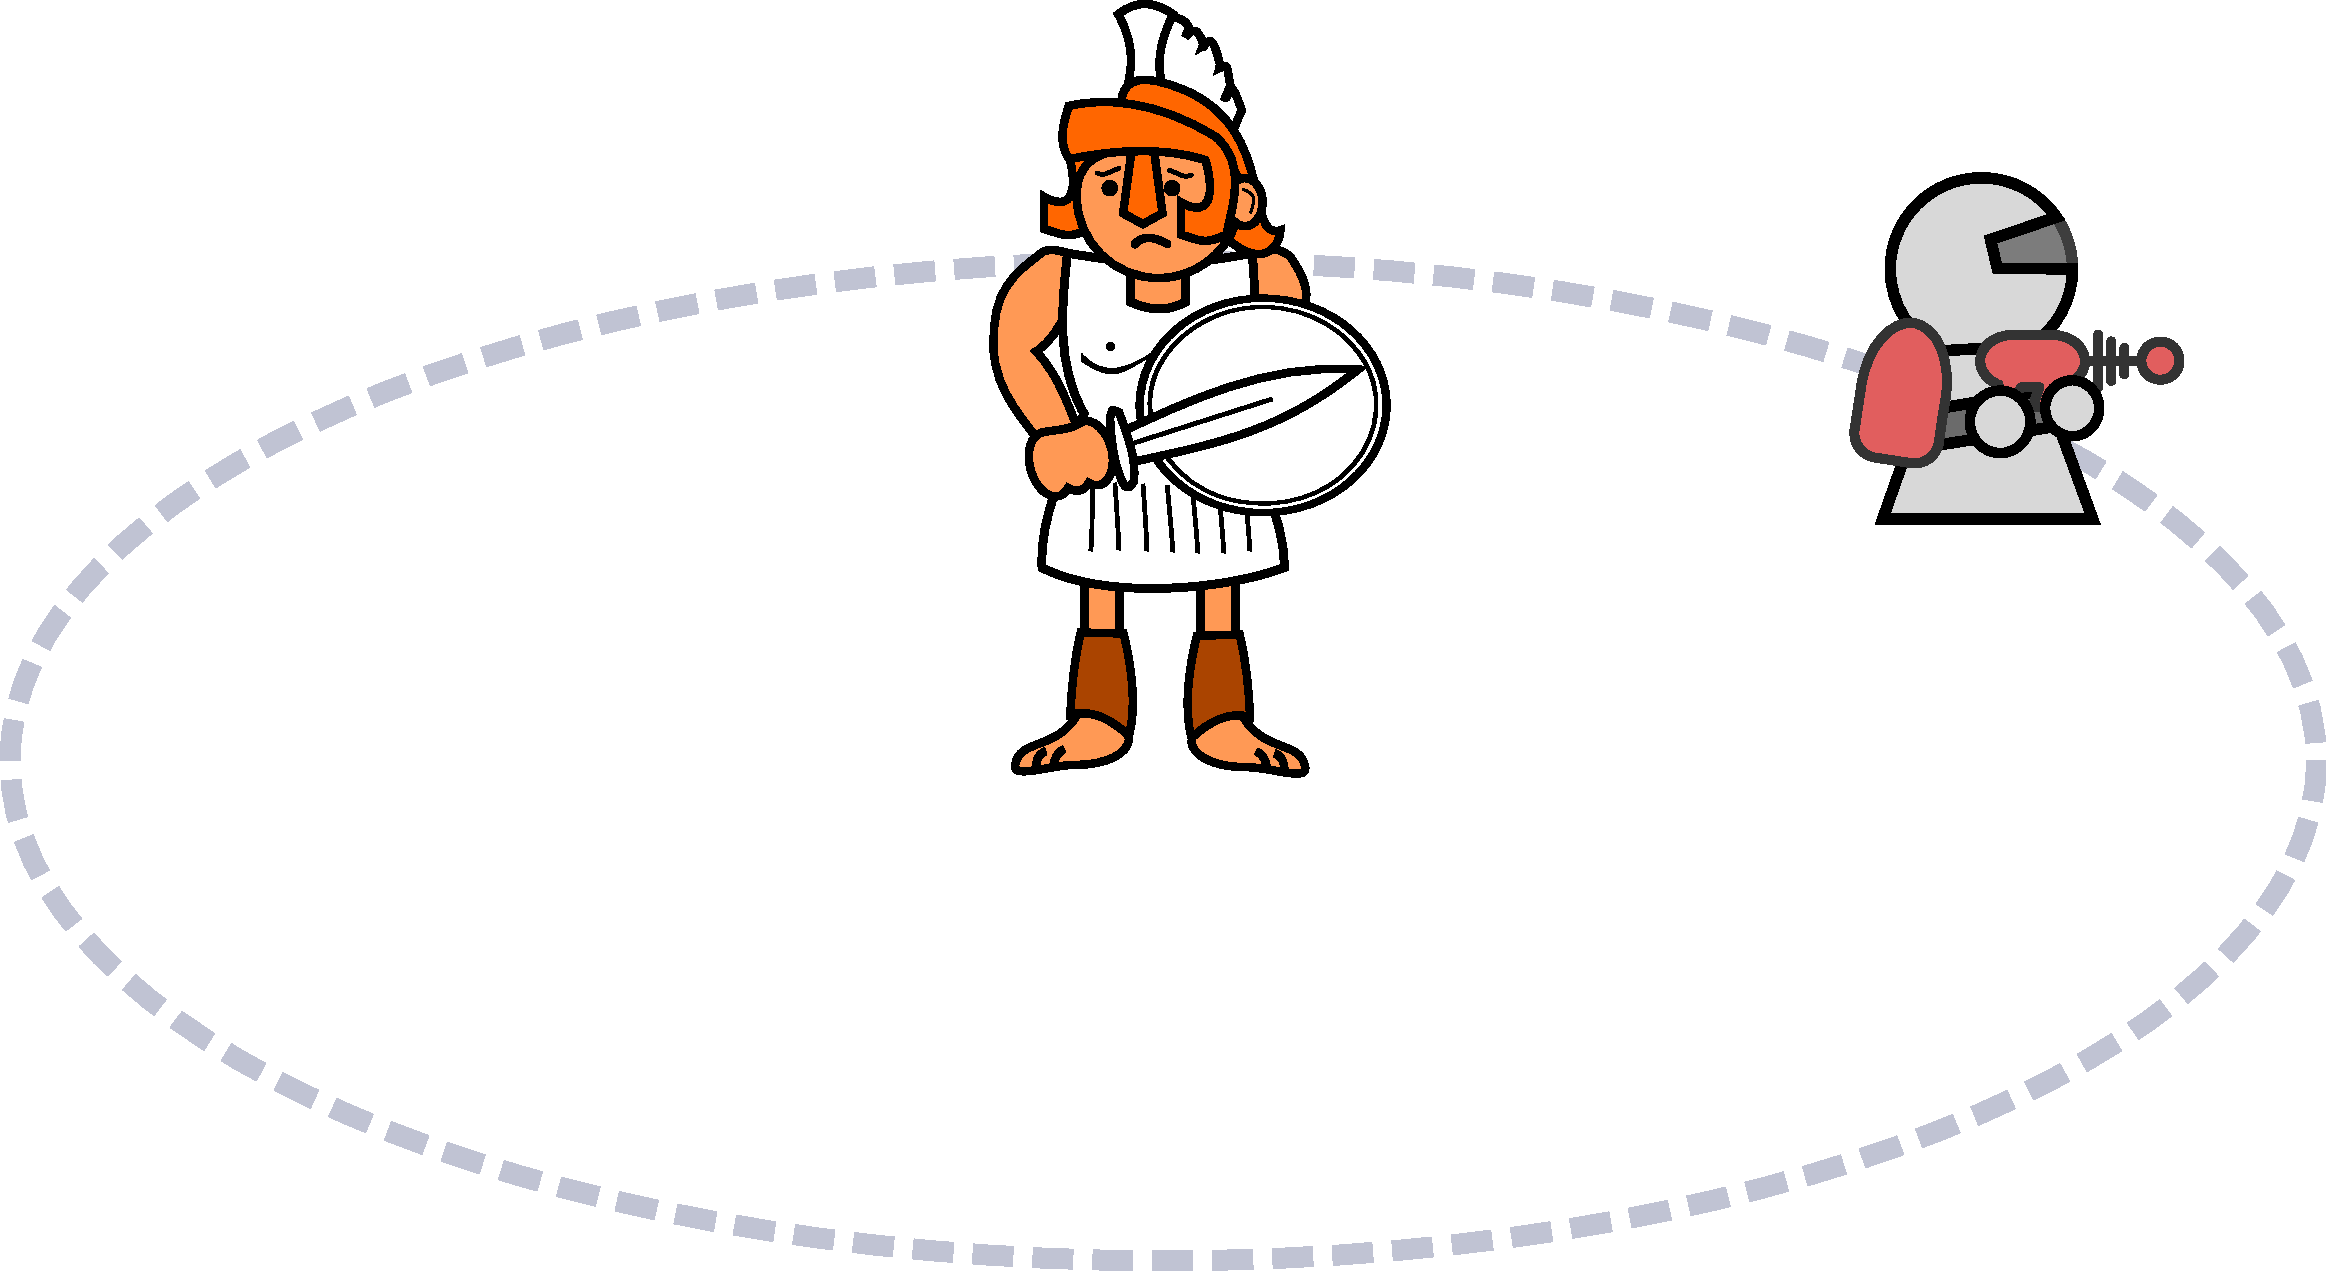
\includegraphics[width = 0.7\textwidth]{./figure/human_robot_interaction}
\end{figure}

\begin{itemize}
\item cooperative observation
\item assistance and protection
\end{itemize}

\end{frame}

\begin{frame}{Neighboring function}{Human constraint}

\begin{columns}
\column{.6\linewidth}
\begin{minipage}[c]{\linewidth}
\begin{figure}
\centering
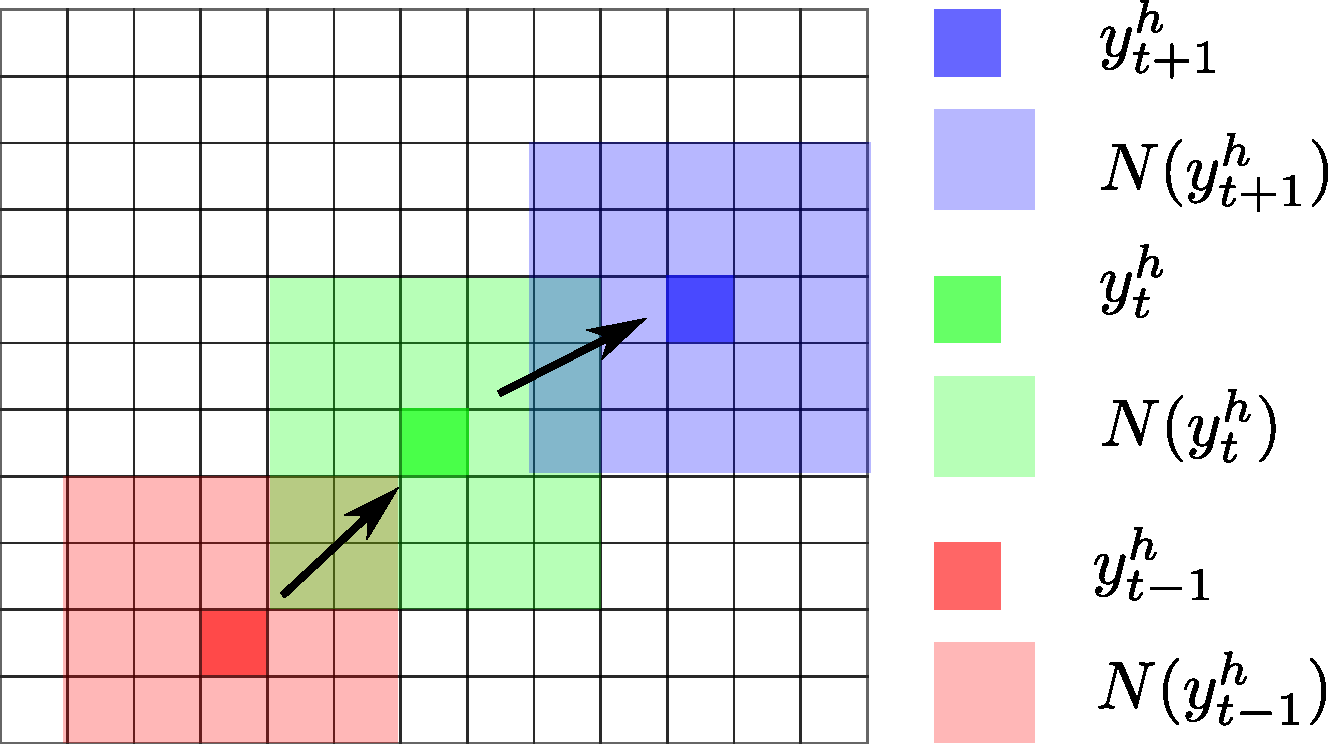
\includegraphics[width = \textwidth]{./figure/humanConstraint}
%\caption{An example of human constraint.}
\end{figure}
\end{minipage}

\column{.4\linewidth}
\begin{minipage}[c]{\linewidth}
\begin{itemize}
\item { human path $ \{ y^{h}_{1} \cdots y^{h}_{T} \} $ }
\item { neighboring function $ N( y^{h}_{t} ) $ }
\end{itemize}
\end{minipage}
\end{columns}

\end{frame}

\subsection{The optimization model}

\begin{frame}{Problem abstraction}{The optimization model}

\begin{figure}
\centering
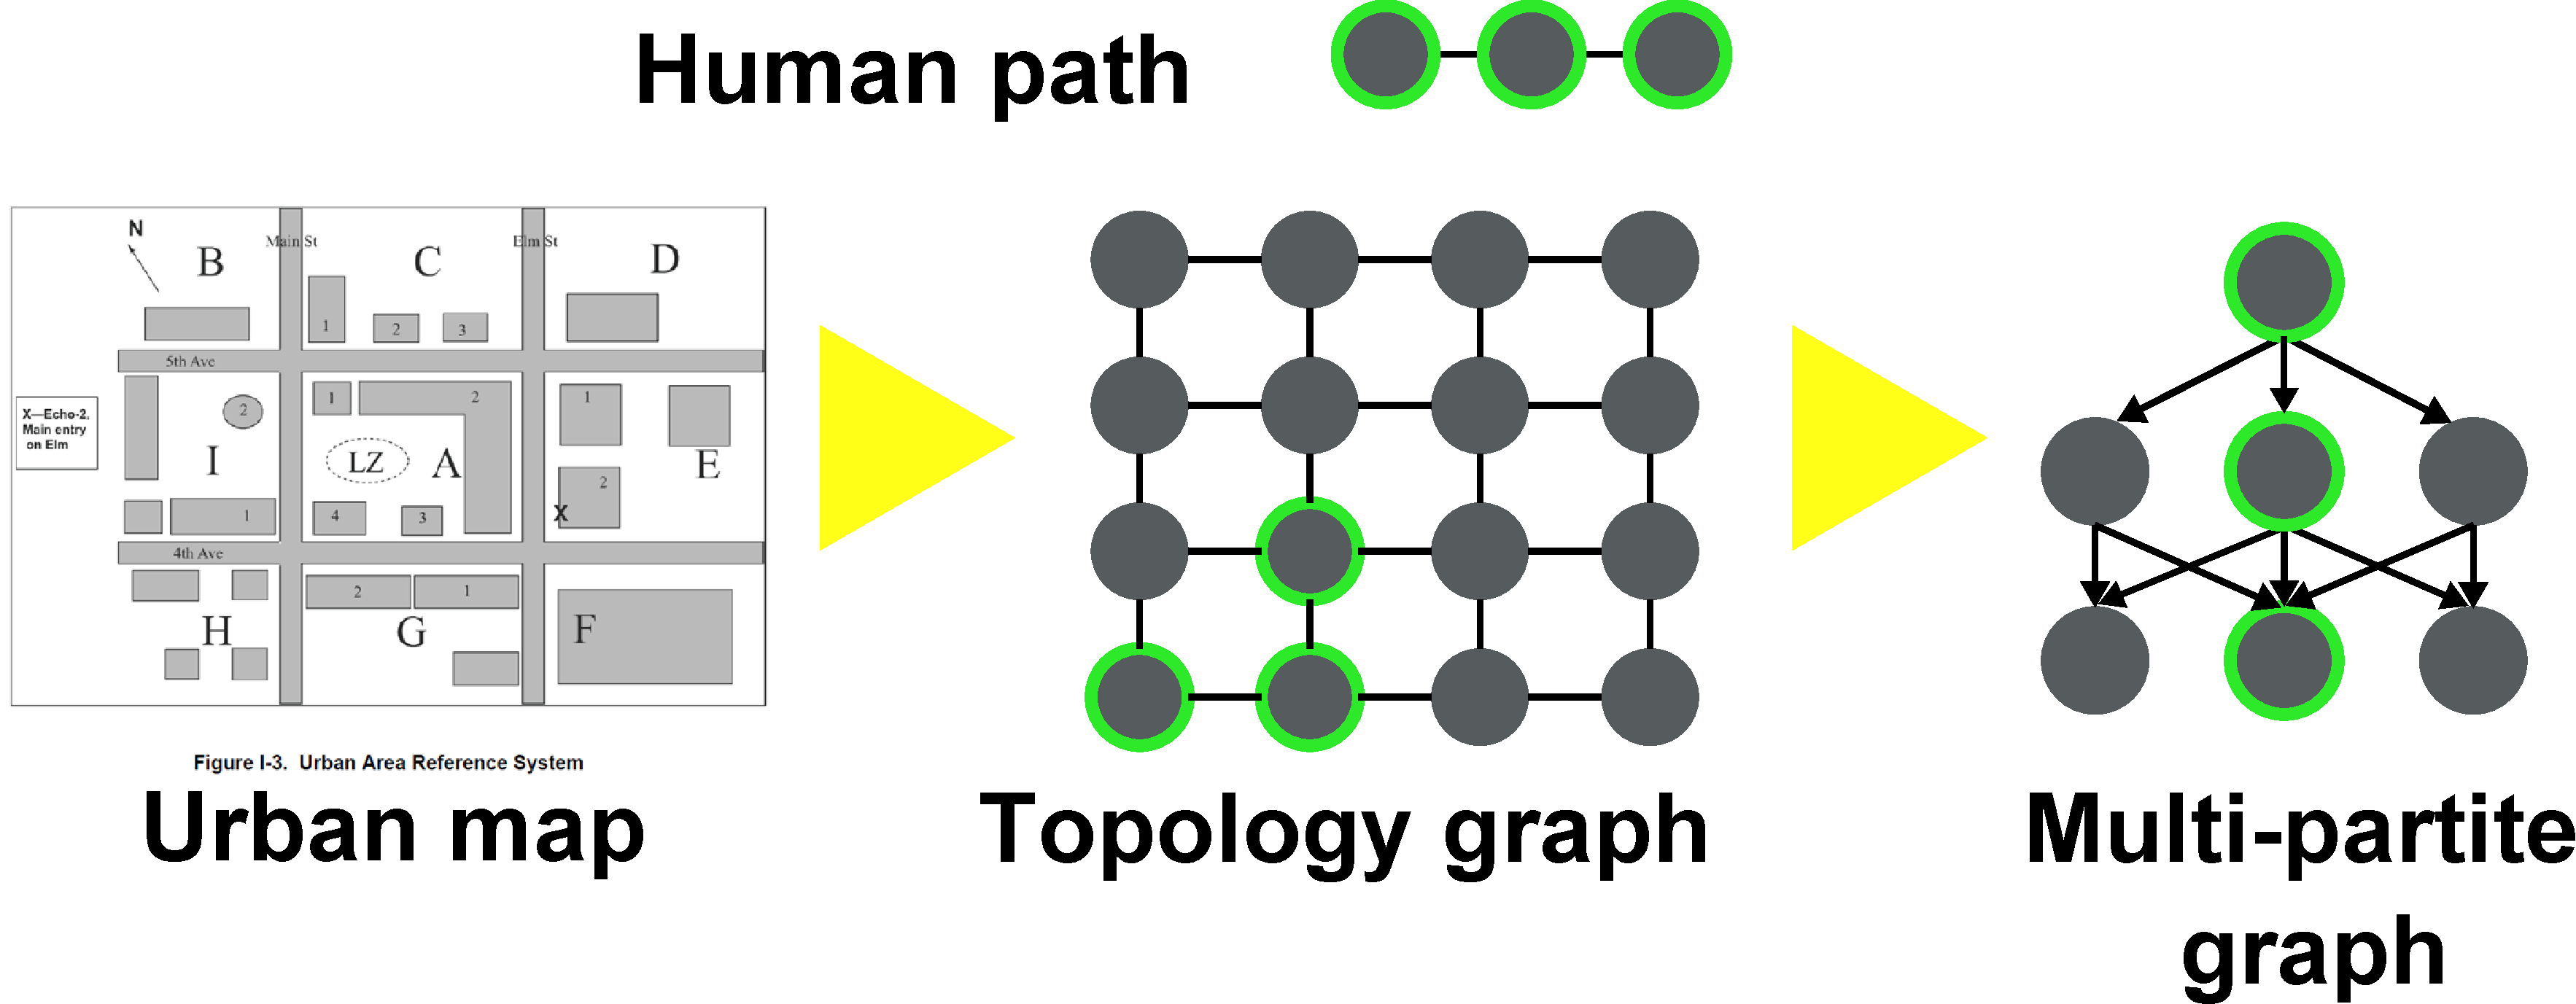
\includegraphics[width = 0.9\textwidth]{./figure/layers}
%\caption{A layered problem processing.}
\end{figure}

\end{frame}

\begin{frame}{The multi-partite graph}{The optimization model}

\begin{columns}

\column{.6\textwidth}
\begin{minipage}[c]{\textwidth}
\begin{figure}
\centering
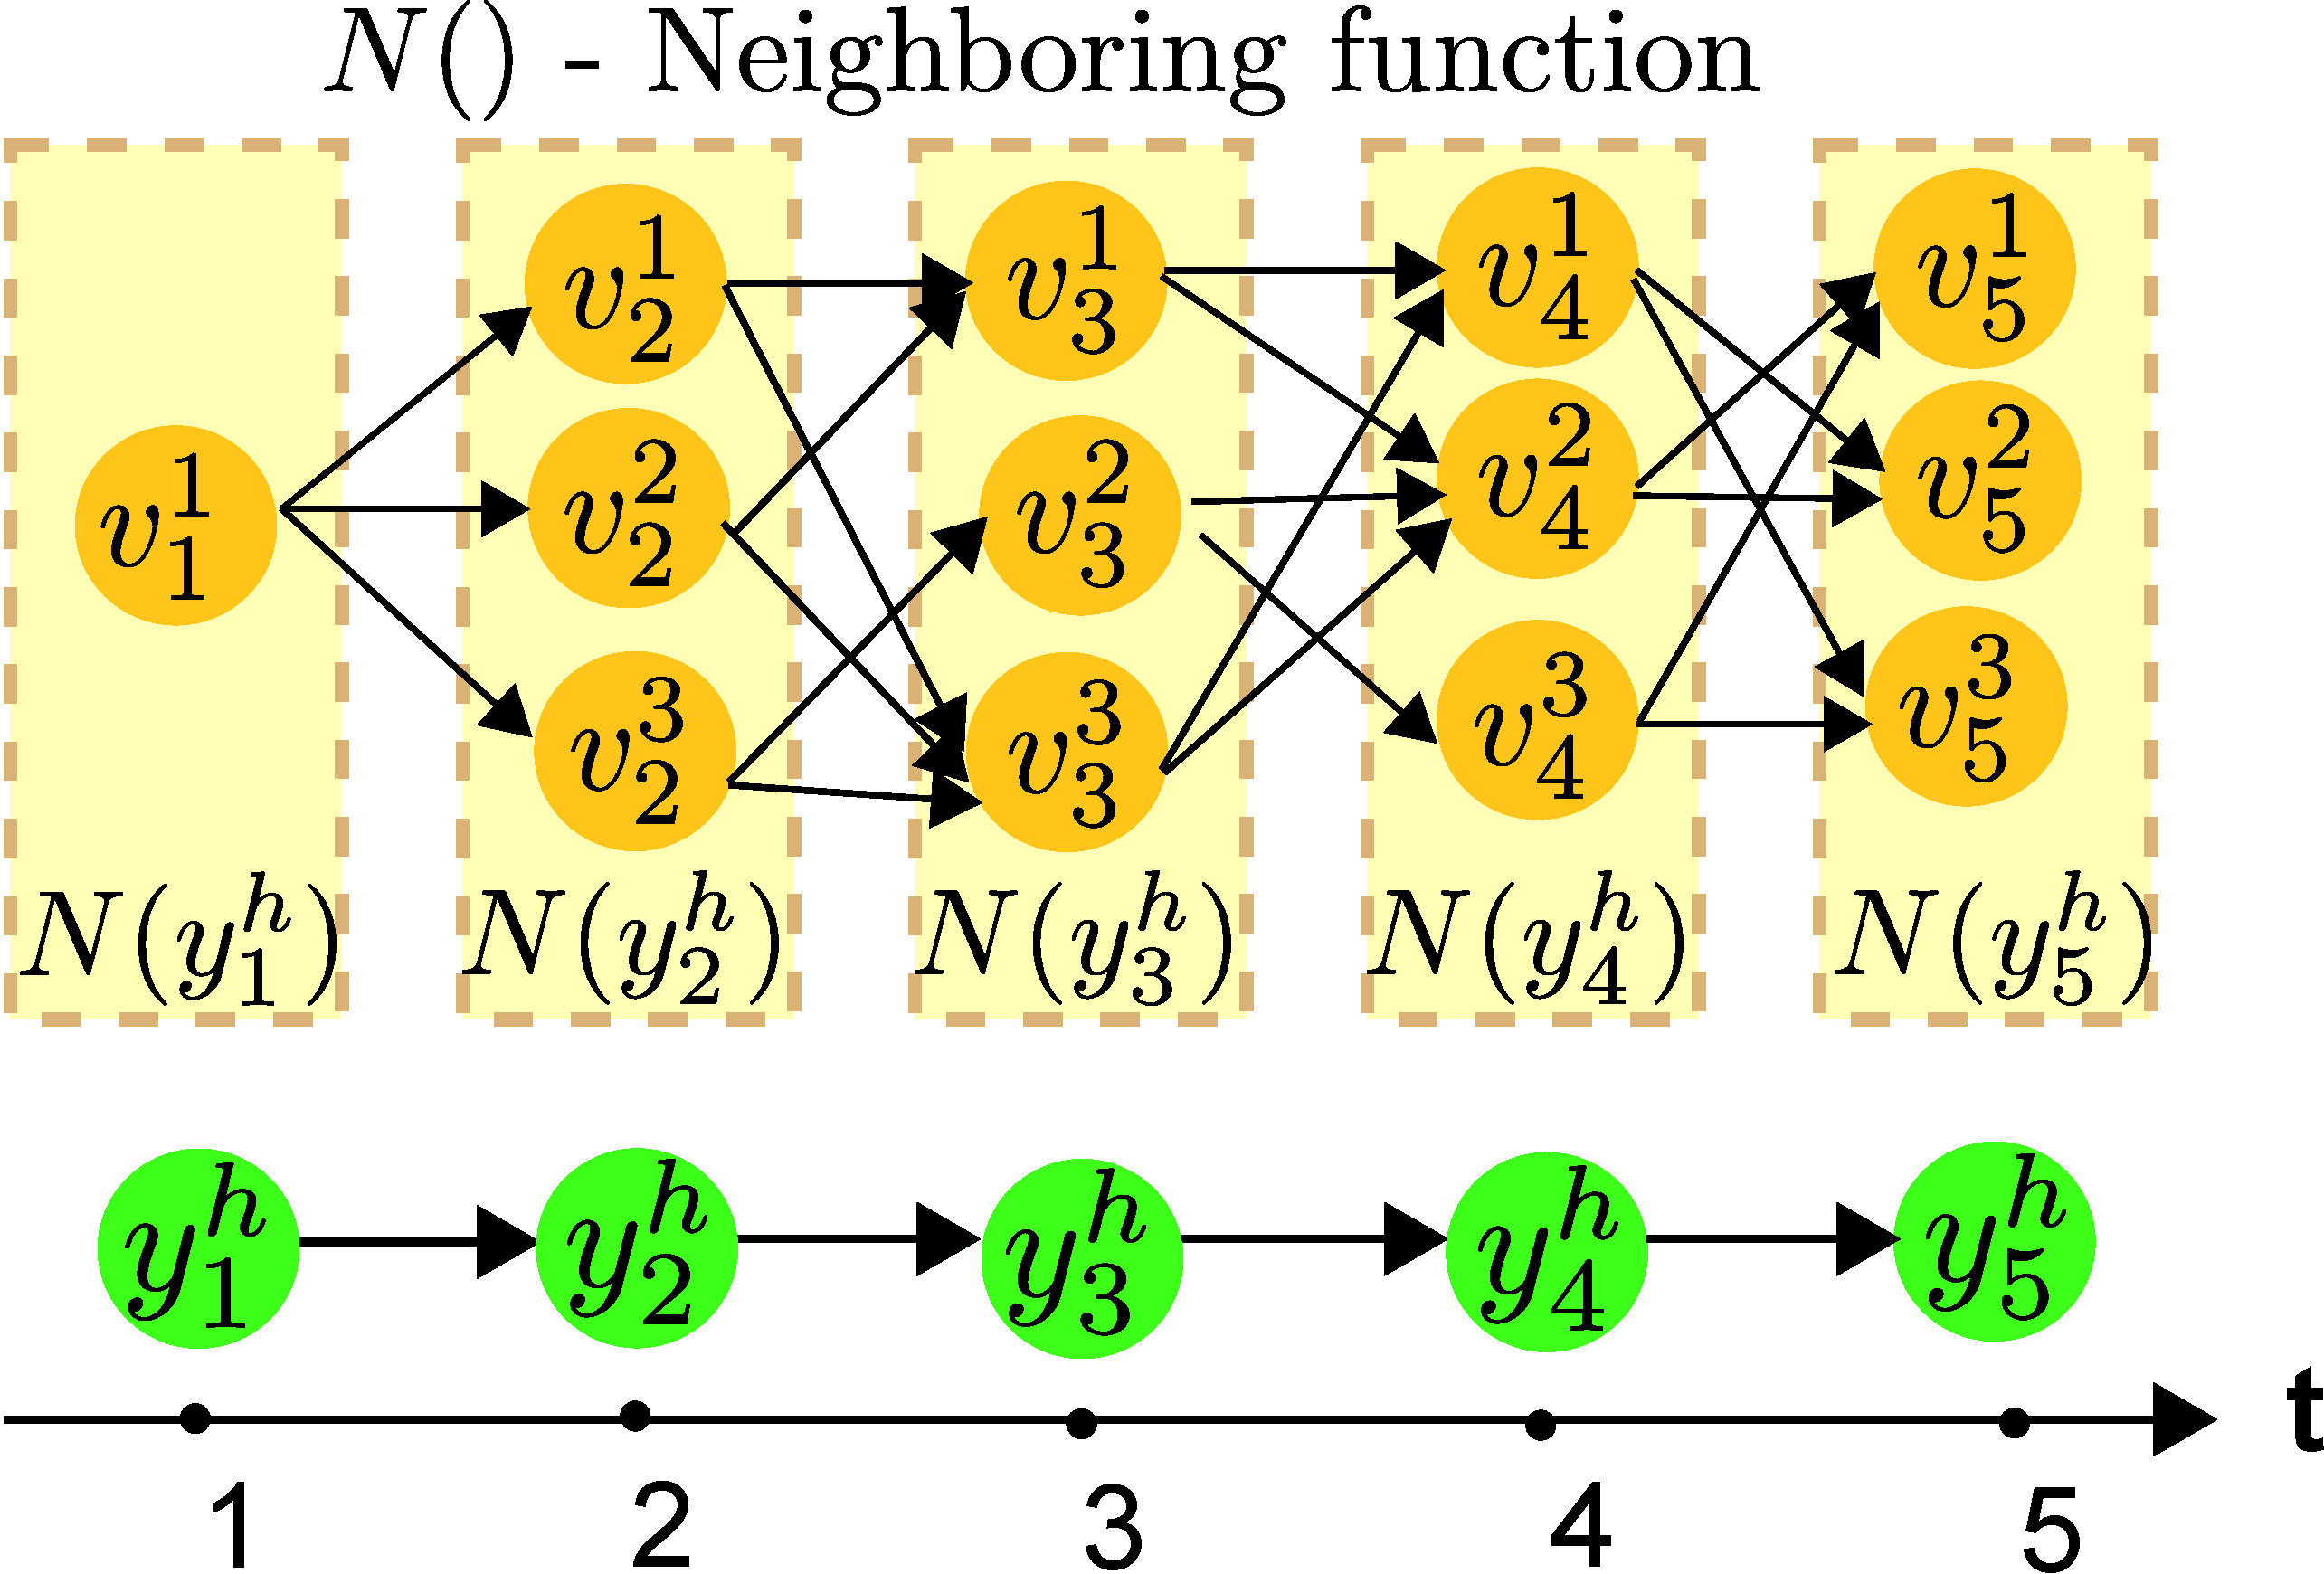
\includegraphics[width = \textwidth]{./figure/MultiPartite}
%\caption{A multi-partite graph generated from human constraint.}
\end{figure}
\end{minipage}

\column{.4\textwidth}
\begin{minipage}[c]{\textwidth}
\begin{itemize}
\item time-space synchronization
\item connection determined by discretized map
\end{itemize}
\end{minipage}

\end{columns}

\end{frame}

\begin{frame}{A pruning process}{The optimization model}

\begin{columns}
\column{.45\textwidth}
%\begin{minipage}
%\begin{block}
Reachable
%\end{block}
%\end{minipage}

\column{.45\textwidth}
%\begin{minipage}
%\begin{block}
Non-terminating
%\end{block}
%\end{minipage} 

\end{columns}

\begin{columns}

\column{.45\textwidth}

\begin{block}{Forward pruning}
$ \forall t \in \{ 2, \cdots T \}, $ \\
$ \forall v \in V(t), deg^{-}(v) > 0 $

\begin{figure}
\centering
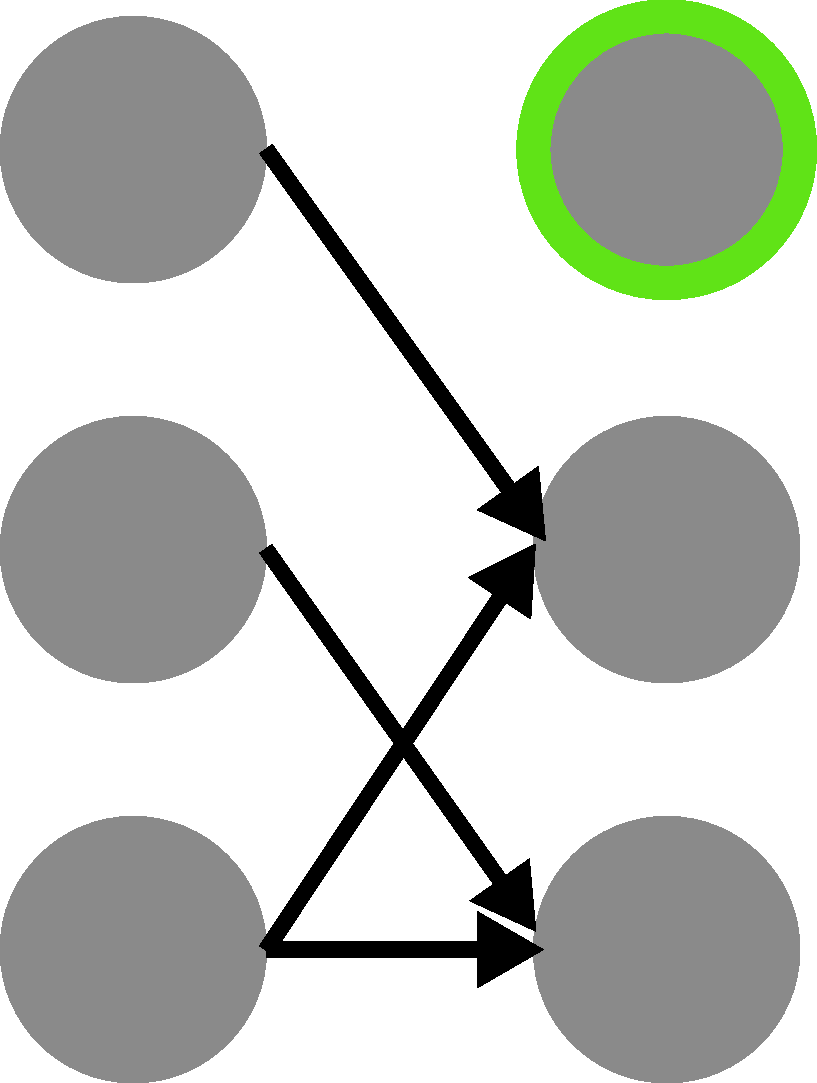
\includegraphics[width = 0.4\textwidth]{./figure/forward_prune}
\end{figure}

\end{block}

\column{.45\textwidth}

\begin{block}{Backward pruning}

$ \forall t \in \{ 1, \cdots T-1 \}, $ \\
$ \forall v \in V(t), deg^{+}(v) > 0 $

\begin{figure}
\centering
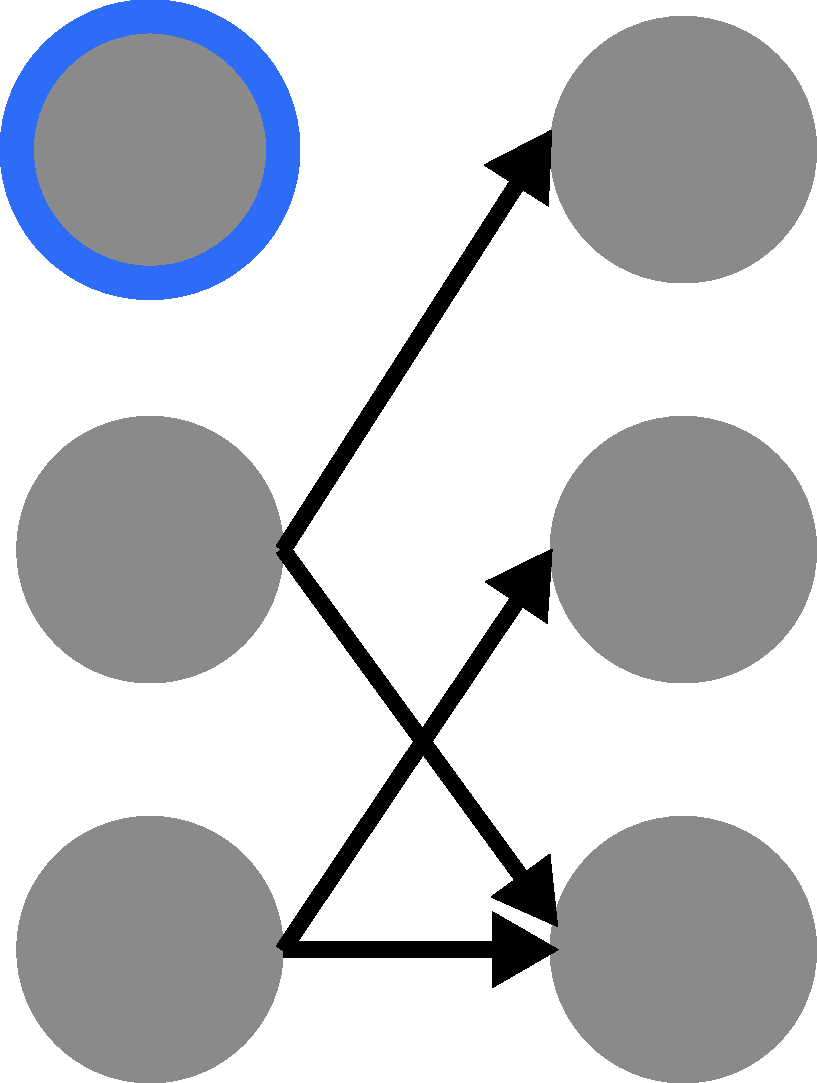
\includegraphics[width = 0.4\textwidth]{./figure/backward_prune}
\end{figure}

\end{block}

\end{columns}

\end{frame}

\begin{frame}{Obstacles}{The optimization model}

\begin{figure}
\centering
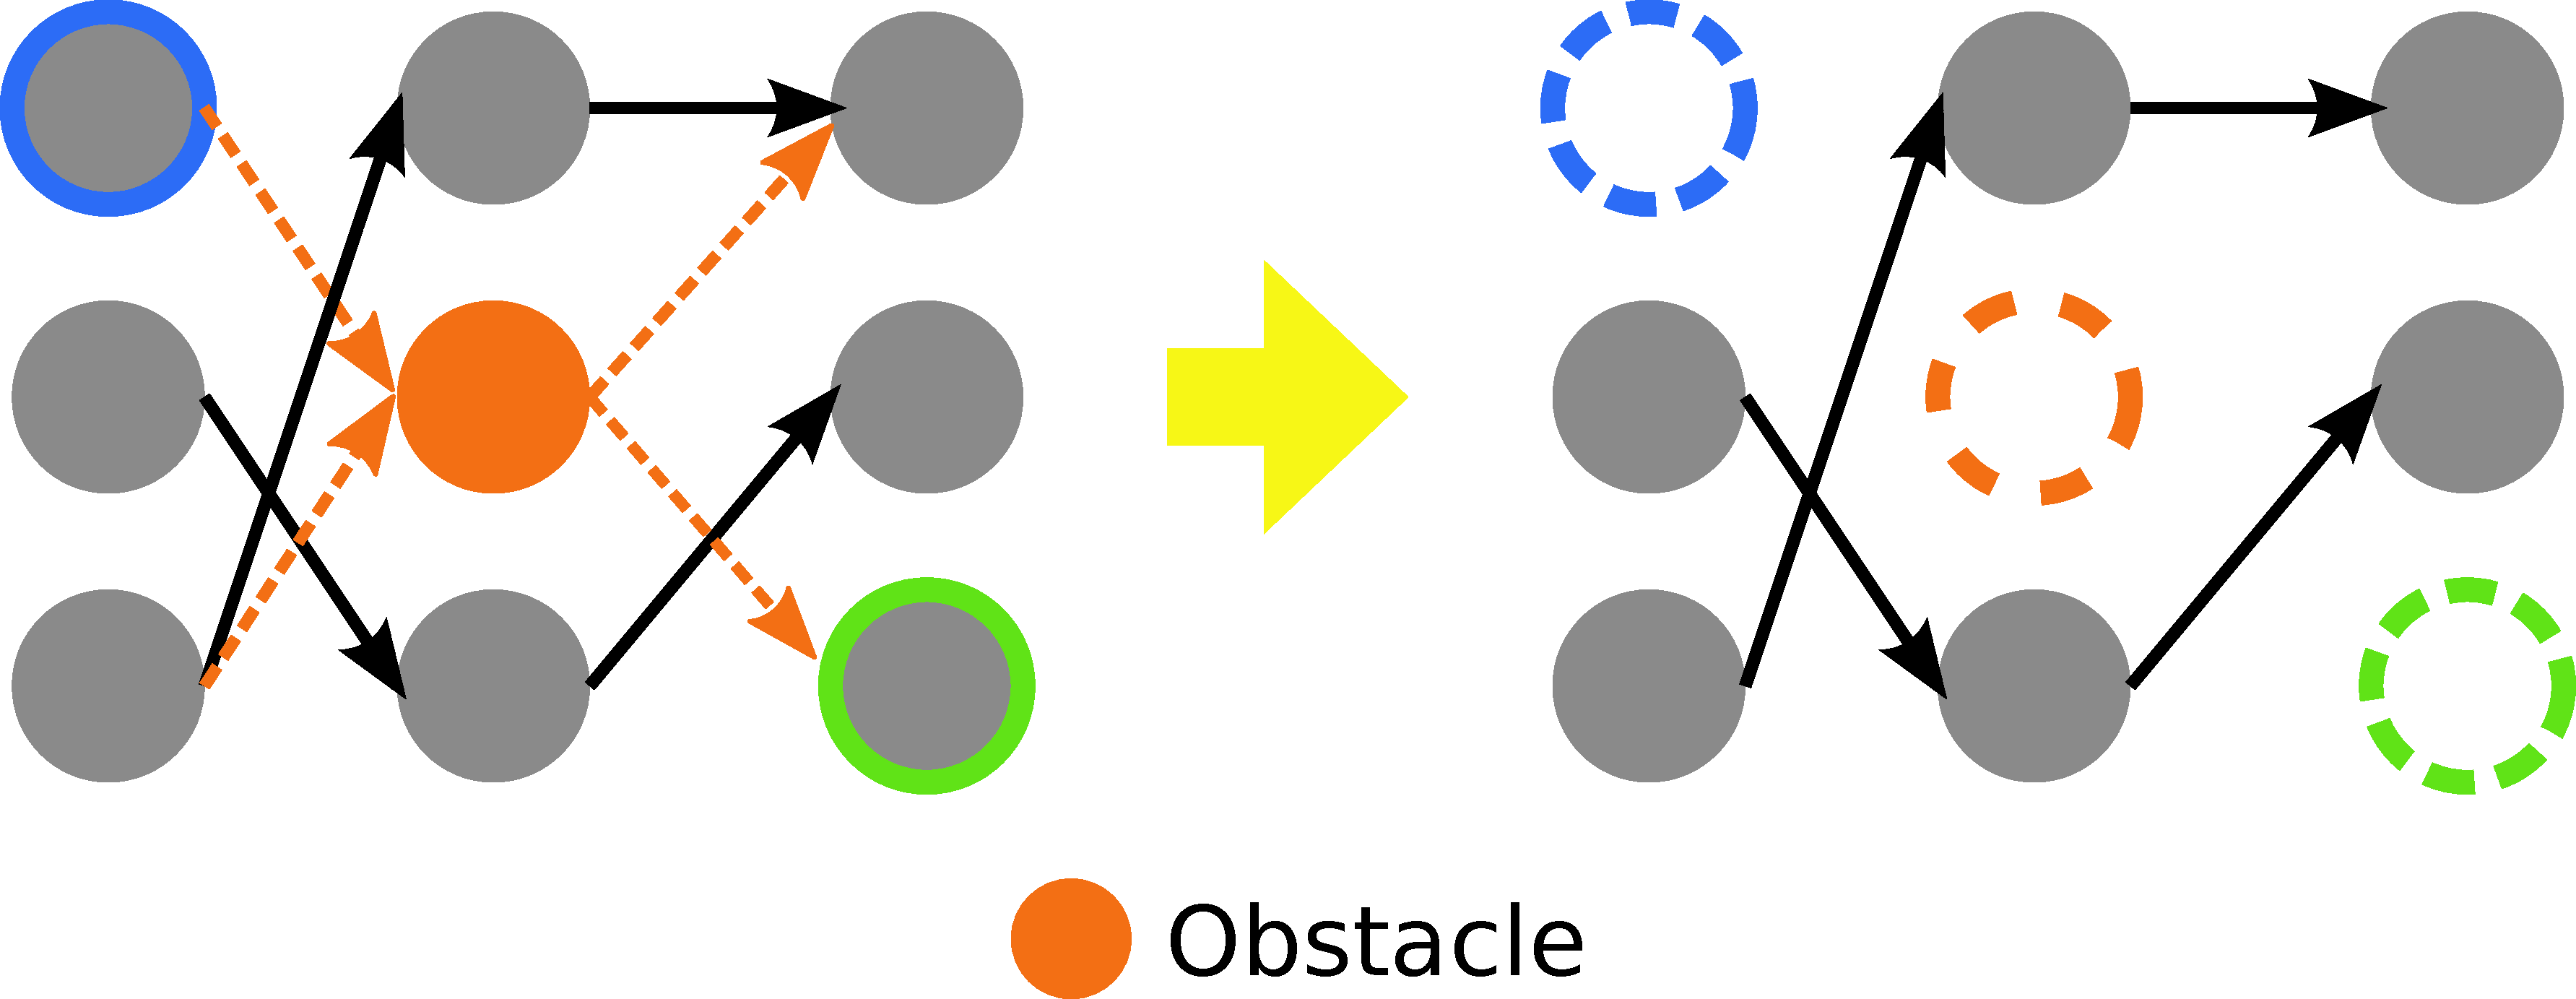
\includegraphics[width = 0.8\textwidth]{./figure/obstacle}
\end{figure}

\end{frame}

\begin{frame}{Submodular orienteering on a multi-partite graph}{The optimization problem}

\begin{equation}
\nonumber
\begin{aligned}
Objective: & X^{*} = \argmax_{X} \: f(X); \\
Constraint: & |X| = T, x_{t} \in V(t), (x_{t}, x_{t+1}) \in E.
\end{aligned}
\end{equation}

\end{frame}



\section{Solution}

\subsection{Backtracking heuristic}

\begin{frame}{Bellman-like equation}{Heuristic}

%\begin{equation}
%\nonumber
%\hat{x}_{t} = \argmax_{X_{t}} [ f(x_{t} \mid x_{1} , \cdots , x_{t-1}) + \max_{X_{t+1}, \cdots , X_{T}} f(x_{t+1}, \cdots , x_{T} \mid x_{1}, \cdots , x_{t}) ]
%\end{equation}

\centering
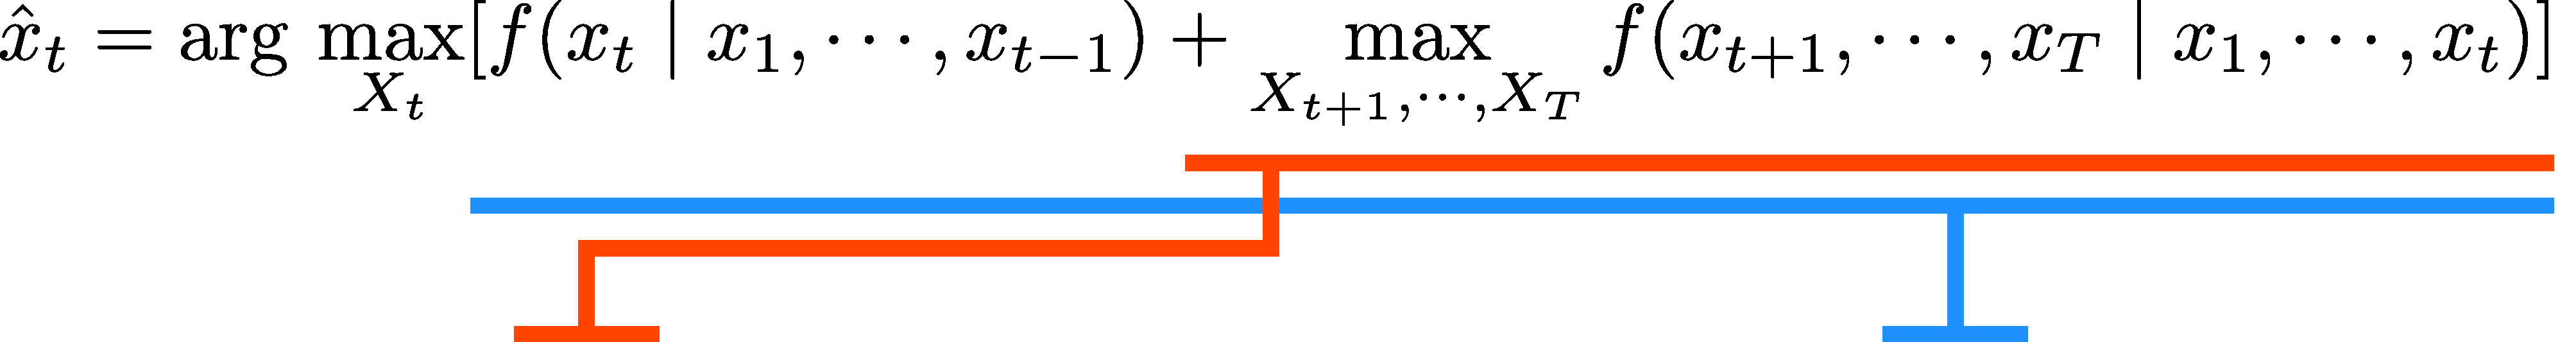
\includegraphics[width = \textwidth]{./figure/arg_equation}

\begin{columns}
\column{0.45\textwidth}
\begin{block}{Maximum future reward}
\begin{figure}
\centering
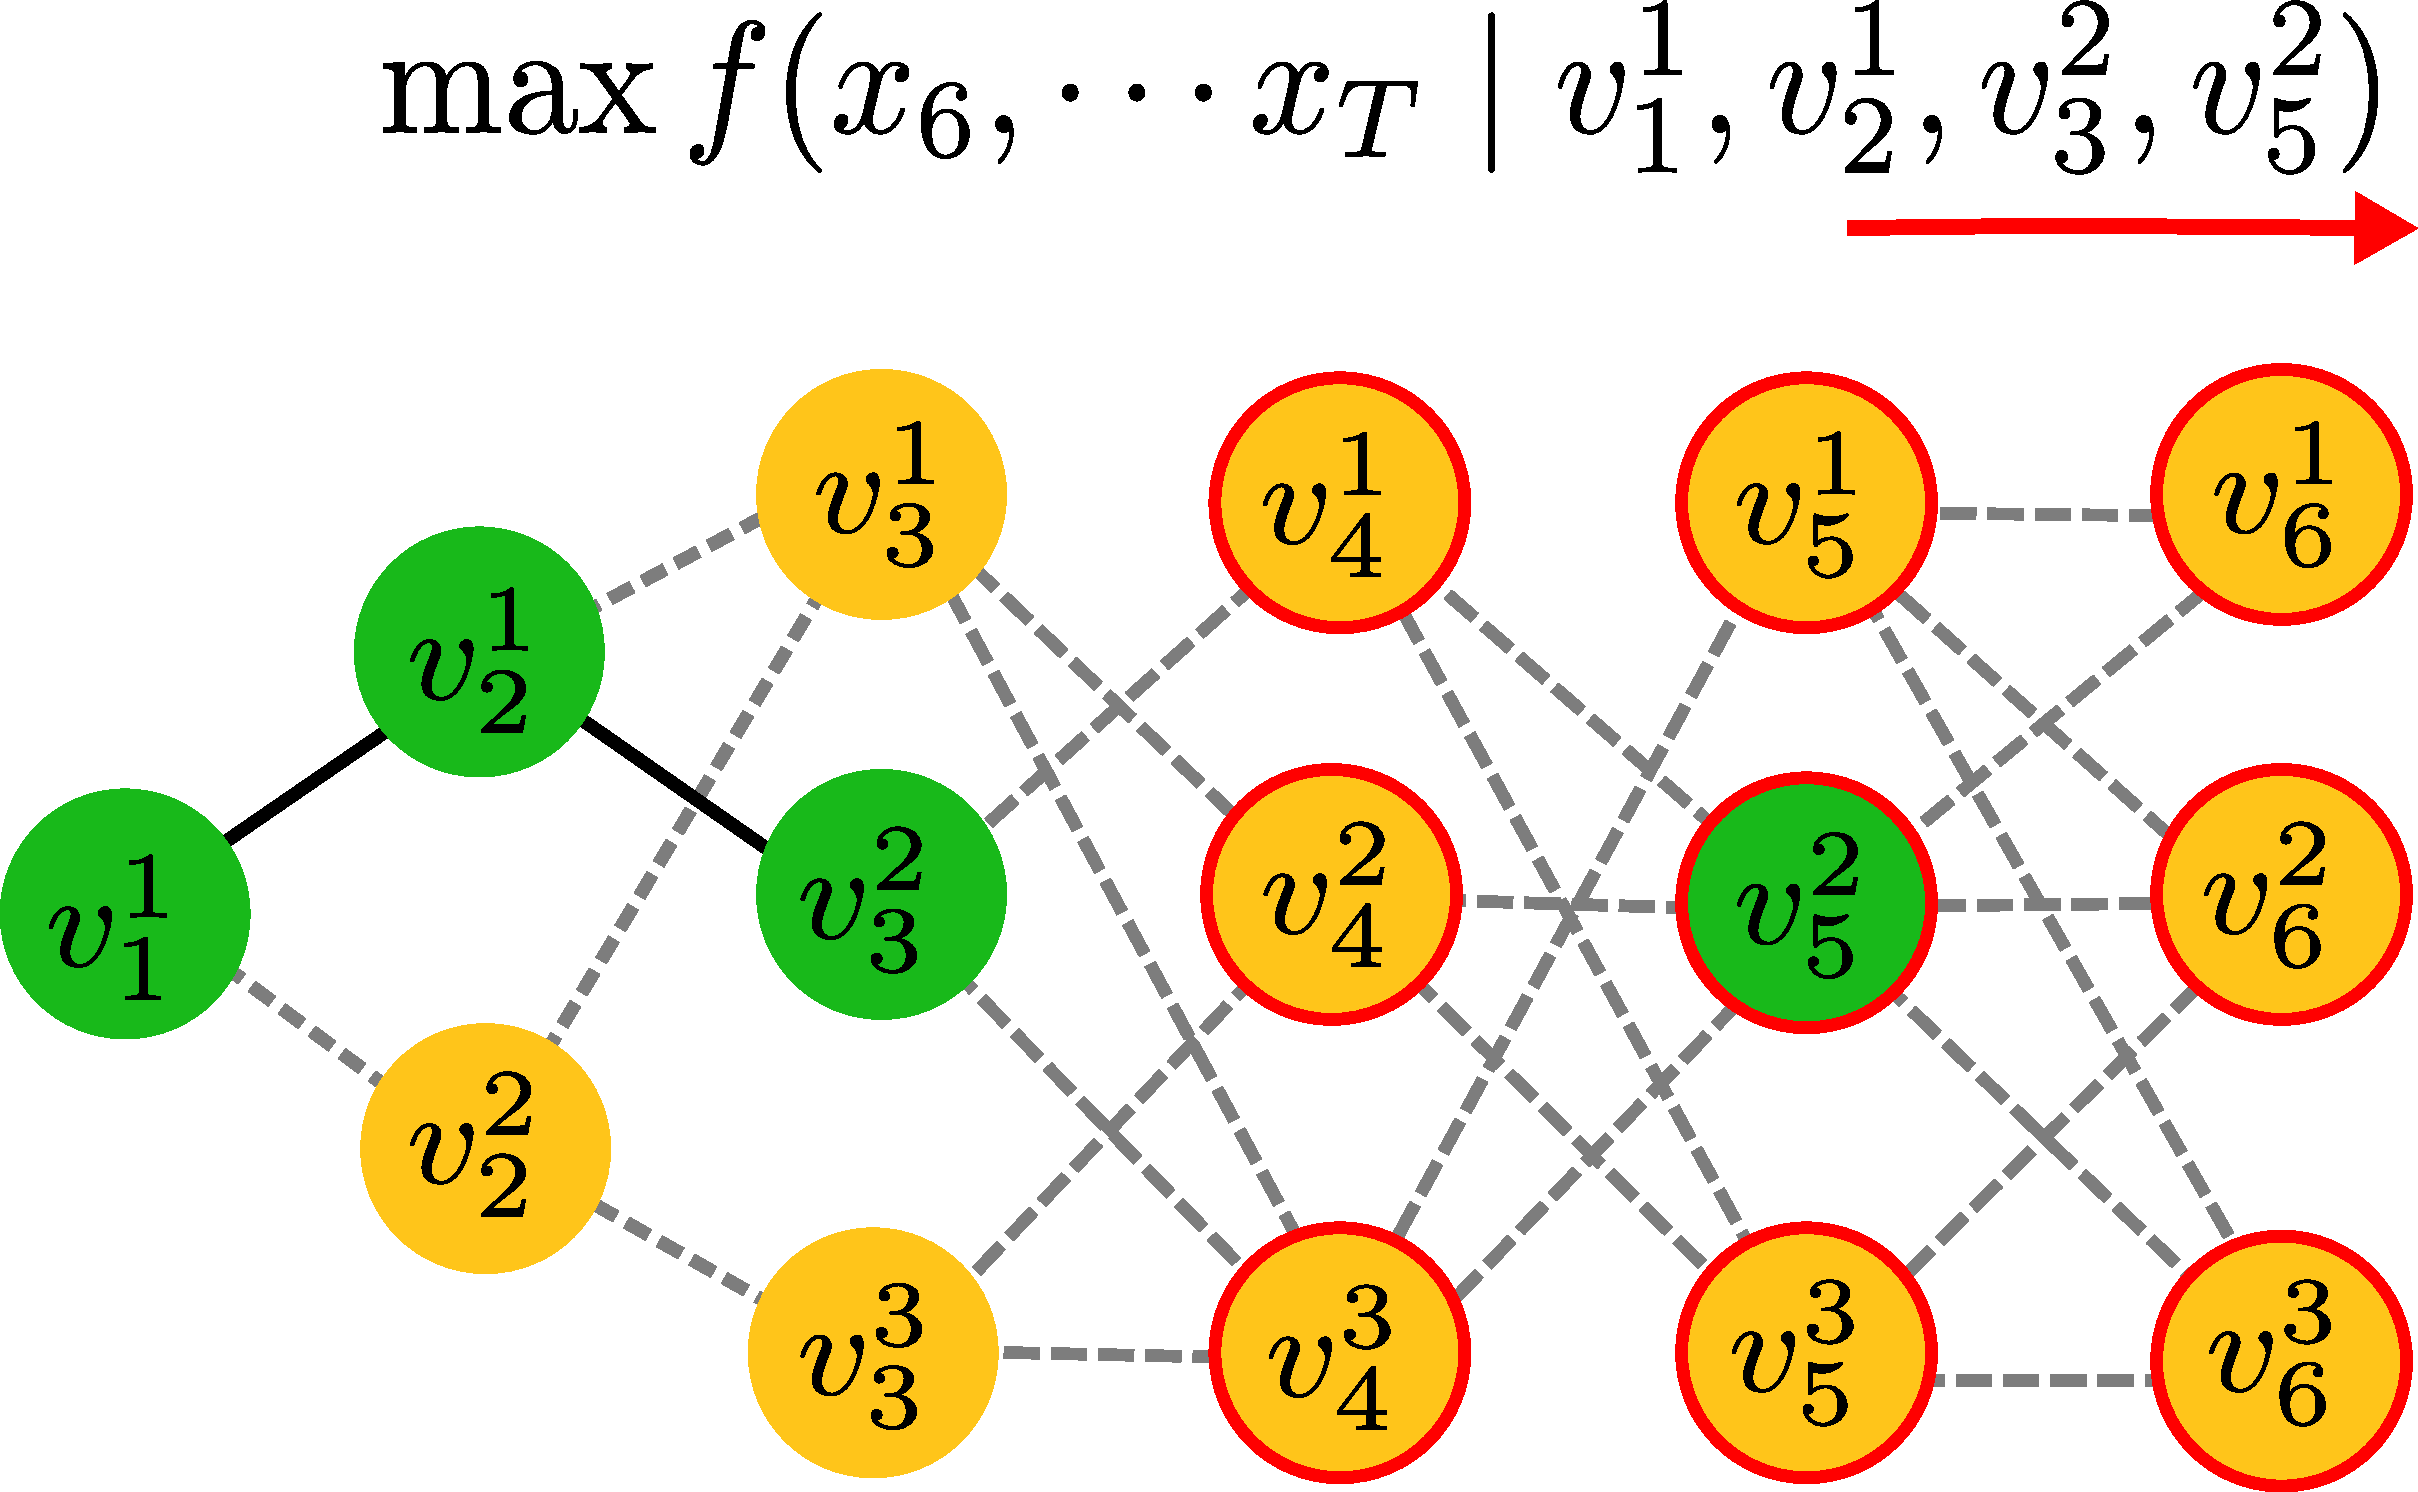
\includegraphics[width = 0.9\textwidth]{./figure/DefineFuncH}
\end{figure}
\end{block}

\column{0.45\textwidth}
\begin{block}{Maximum total reward}
\begin{figure}
\centering
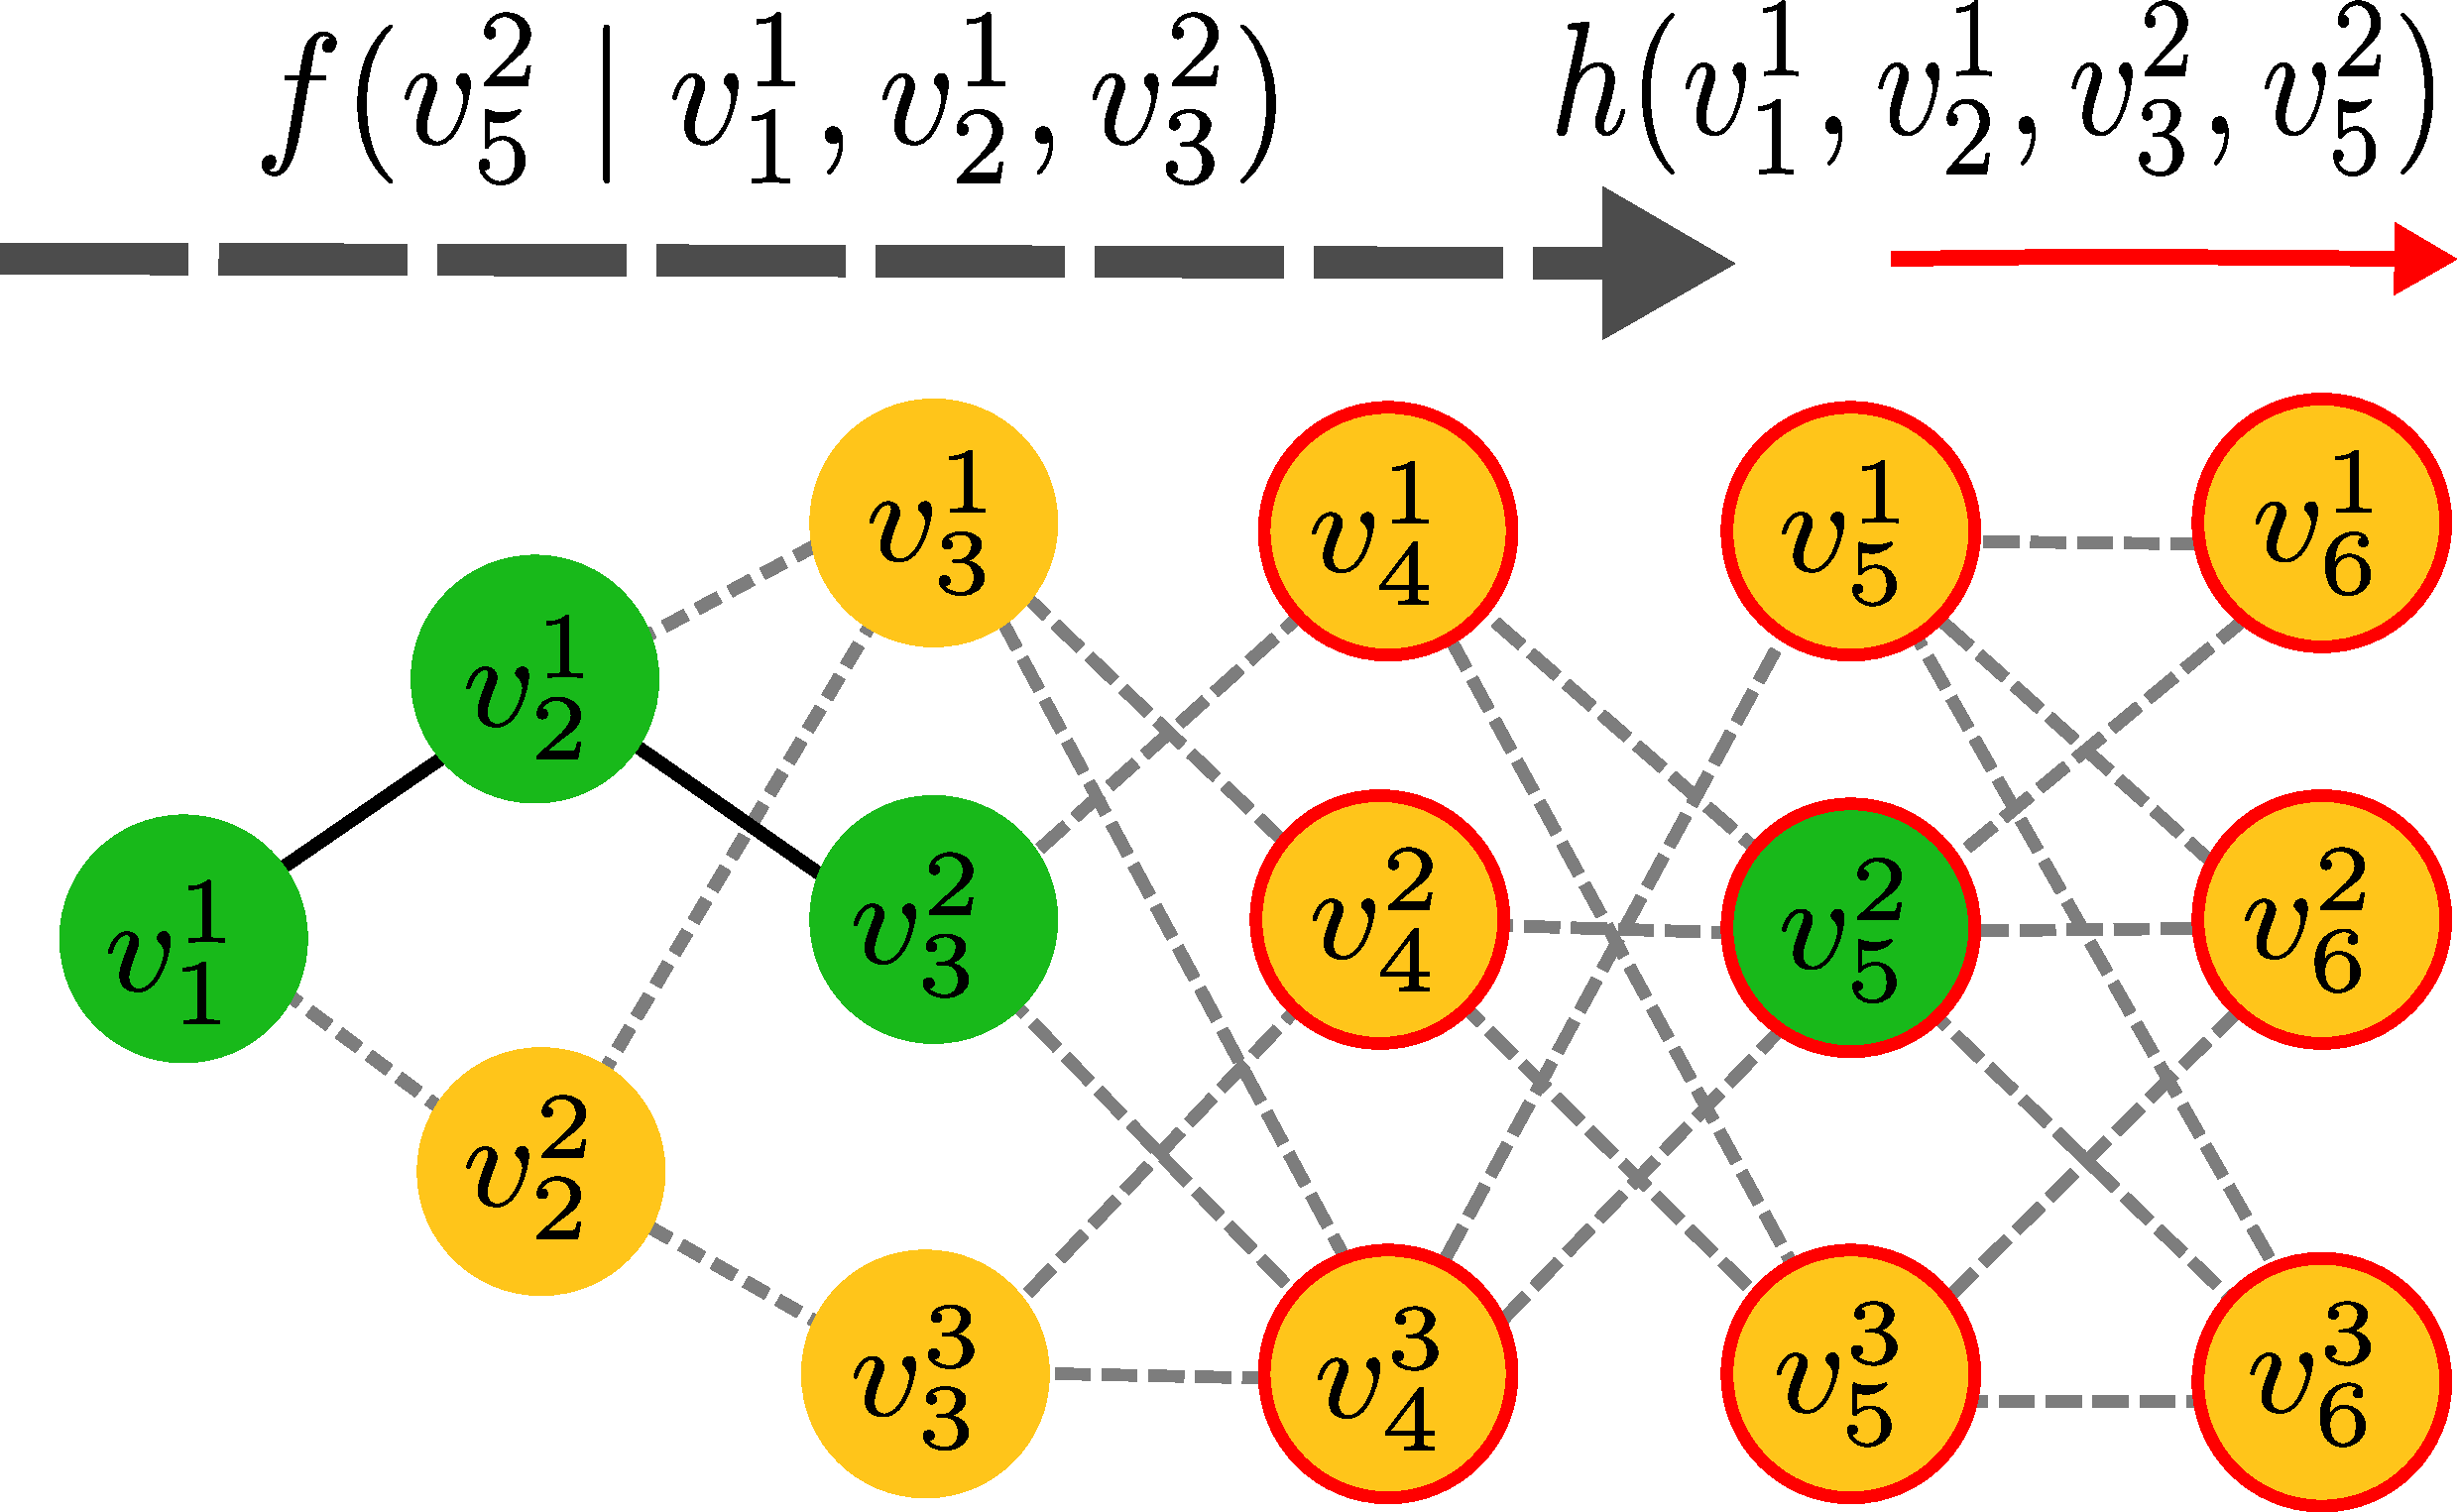
\includegraphics[width = 0.9\textwidth]{./figure/DefineFuncP}
\end{figure}
\end{block}
\end{columns}

\begin{figure}
\centering

\includegraphics[width = 0.9\textwidth]{./figure/DefineFuncHelp}
\end{figure}

\end{frame}

\begin{frame}{Backtracking}{Heuristic}

\begin{columns}

\column{0.6\textwidth}
\begin{minipage}{\textwidth}
\begin{figure}
\centering
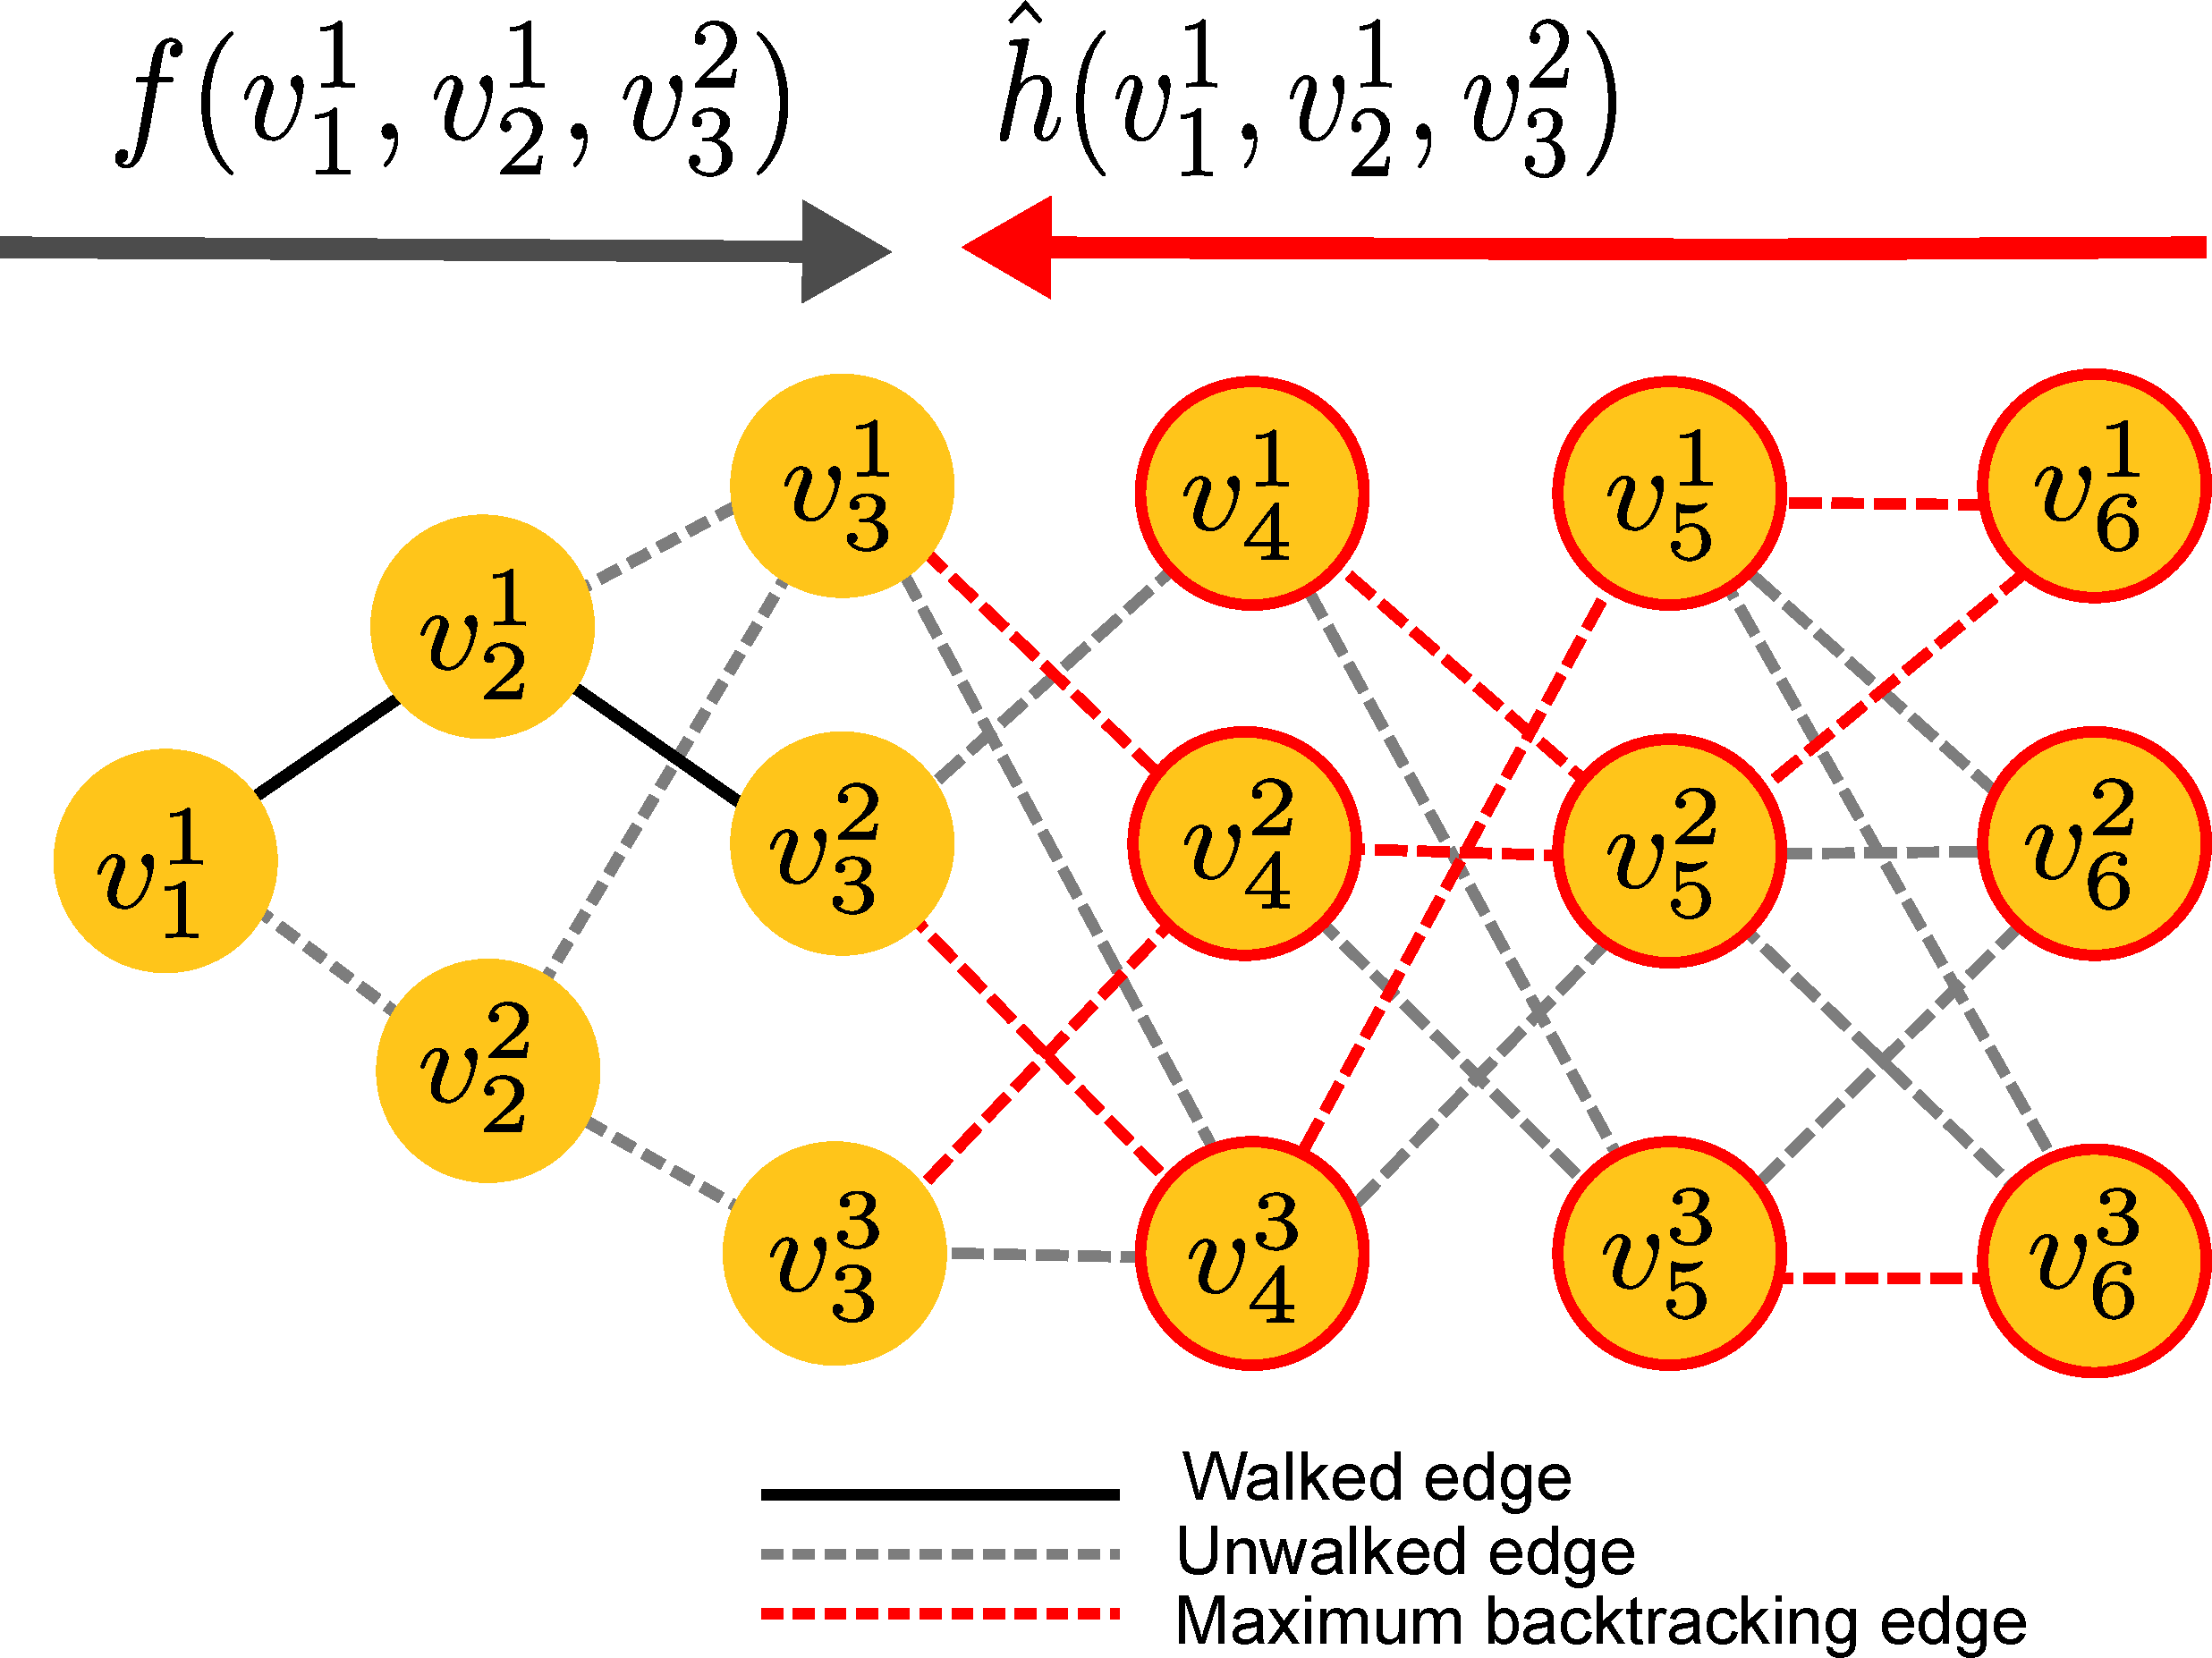
\includegraphics[width = \textwidth]{./figure/backtracking}
\end{figure}
\end{minipage}

\column{0.4\textwidth}
\begin{minipage}{\textwidth}
\begin{itemize}
\item point model $ \rightarrow $ true max total reward
\item coverage model $ \rightarrow $ estimated max total reward guarantee
\end{itemize}
\end{minipage}

\end{columns}

\end{frame}

\subsection{Anytime algorithm design}

\begin{frame}{Expanding tree}{Anytime algorithm framework}

\begin{columns}

\column{0.6\textwidth}
\begin{minipage}{\textwidth}
\begin{figure}
\centering
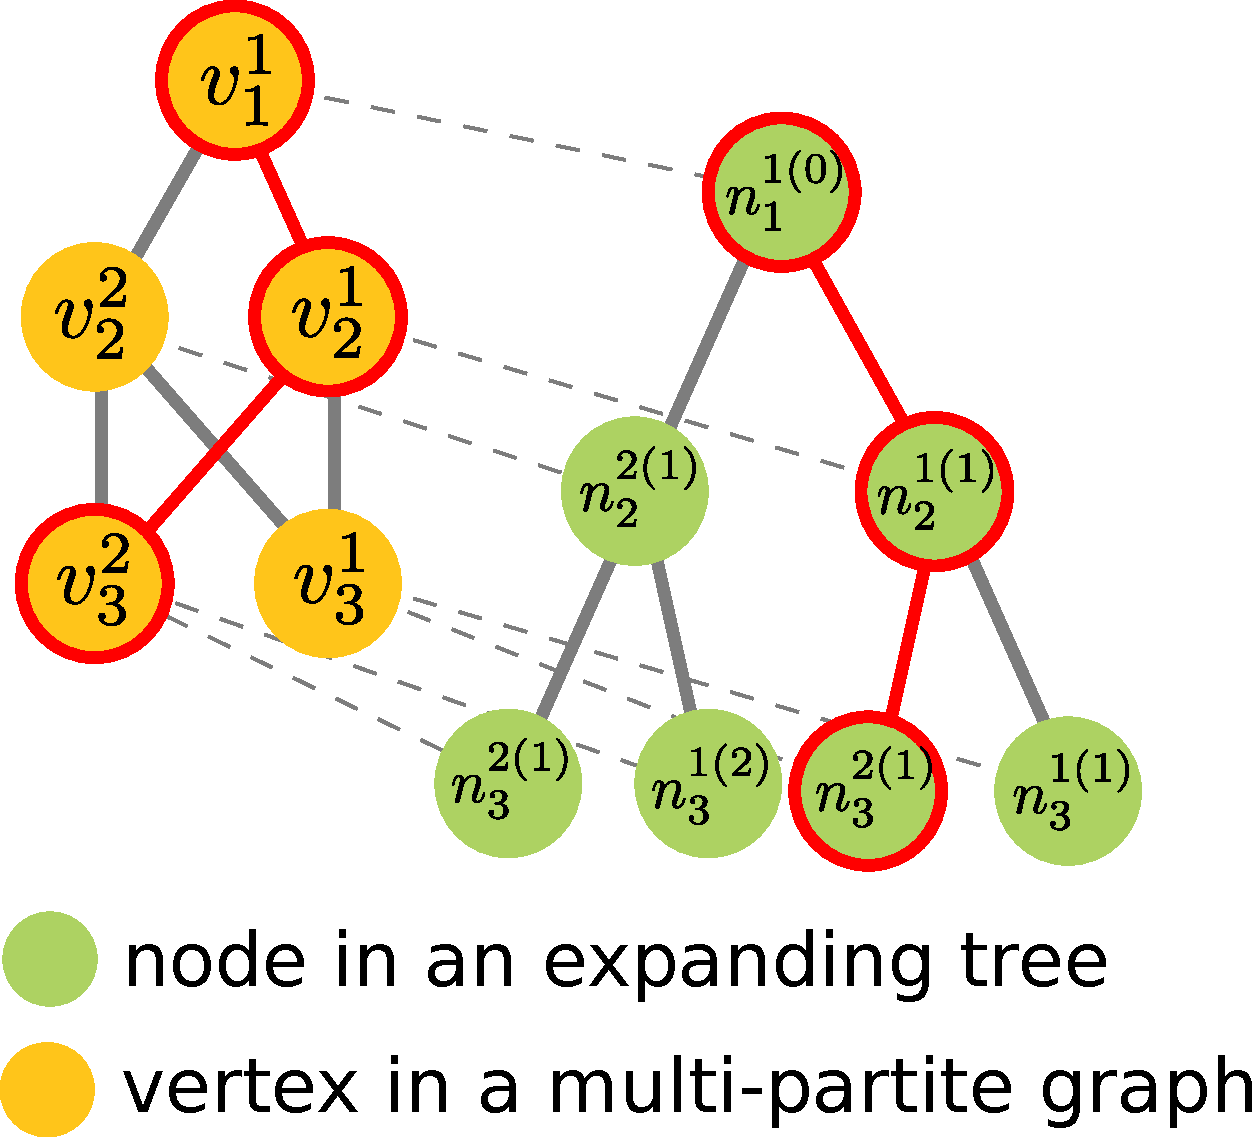
\includegraphics[width=.9\textwidth]{./figure/multipartite_expandingtree}
\end{figure}
\end{minipage}

\column{0.4\textwidth}
\begin{minipage}{\textwidth}
\begin{itemize}
\item depth-first recursive traverse
\item node $ \Longleftrightarrow $ subpath
\item tracking the search process
\item estimation storage
\end{itemize}
%Exapnding tree $ G_{T} = (N, L, T) $ \\
%\begin{itemize}
%\item $ T $ - tree depth
%\item $ N $ - Node set
%\item $ L $ - directed link set
%\end{itemize}
\end{minipage}

\end{columns}

\end{frame}

\begin{frame}{Node freeze}{Anytime algorithm framework}

Estimated reward $ \leq $ Current best reward 
$ \Longrightarrow $ Stop exploring subpath

\begin{figure}
\centering
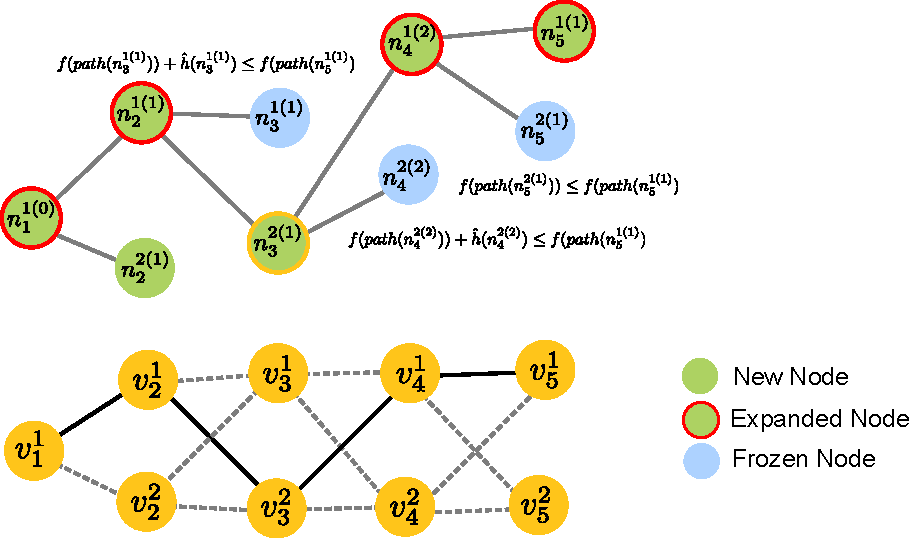
\includegraphics[width =  0.8\textwidth]{./figure/freeze_process}
\end{figure}

\end{frame}

\begin{frame}{Flow}{Anytime algorithm framework}

\begin{figure}
\centering
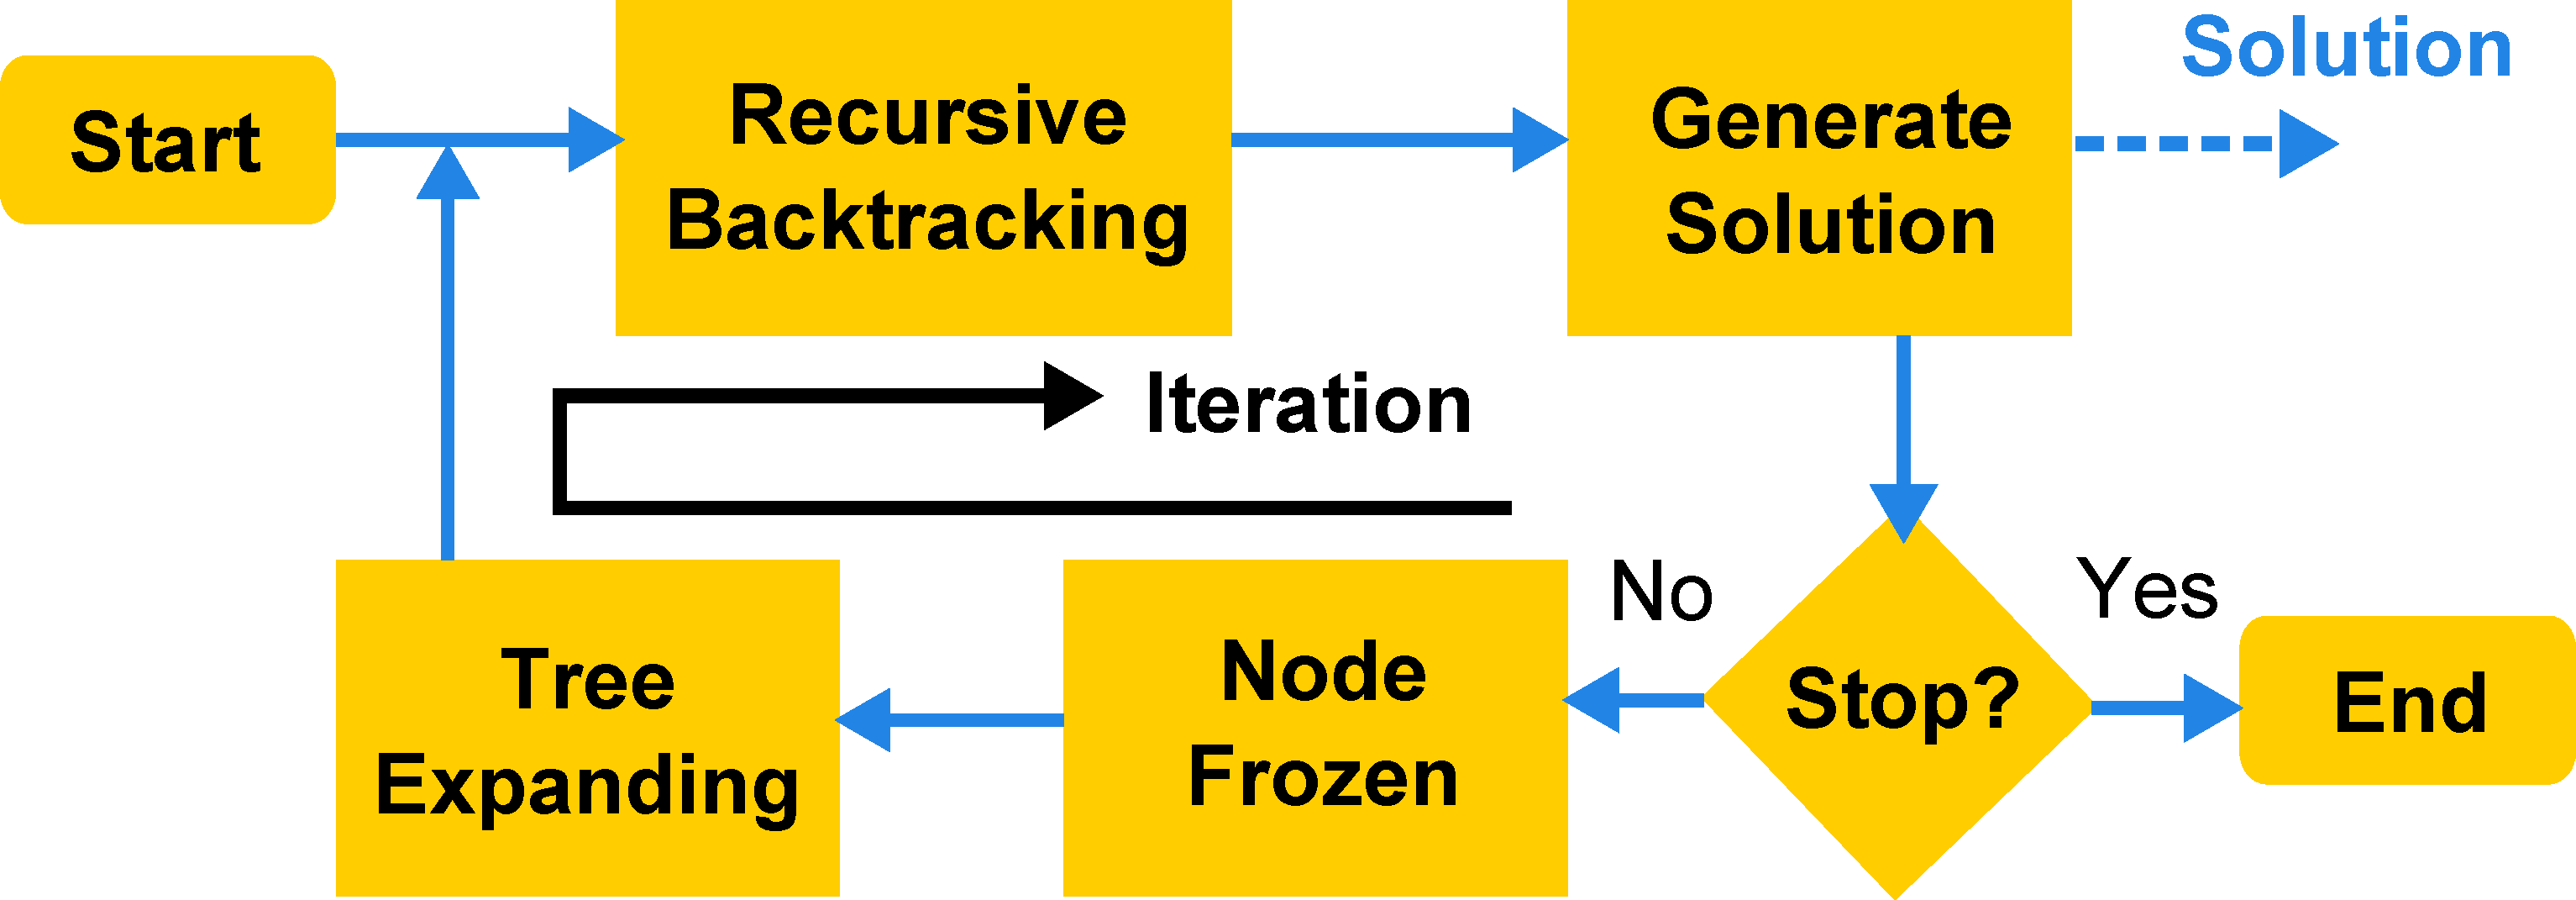
\includegraphics[width = 0.9\textwidth]{./figure/alg_flow}
\end{figure}

\end{frame}

\begin{frame}{Performance guarantee}{Anytime algorithm framework}

\begin{lemma}
“Backtracking” in Algorithm 1 never \textcolor{red}{underestimates}
the maximum total reward, which means
\begin{equation}
\nonumber
\forall t \geq t', \hat{u}(x_{t} \mid v_{1} , \cdots , v_{t'}) \geq u(x_{t} \mid v_{1} , \cdots , v_{t'}).
\end{equation}
\end{lemma}

\begin{minipage}{\textwidth}
\begin{figure}
\centering

\includegraphics[width = 0.15\textwidth]{./figure/arrow}
\end{figure}
\end{minipage}

\begin{theorem}
The anytime algorithm framework in Algorithm 4 can always find an \textcolor{red}{optimal} solution given enough time.
\end{theorem}

\end{frame}

\section{Results}

\subsection{Robot wingman}

\begin{frame}{A robot Wingman problem}{Robot Wingman}

\begin{figure}
\centering
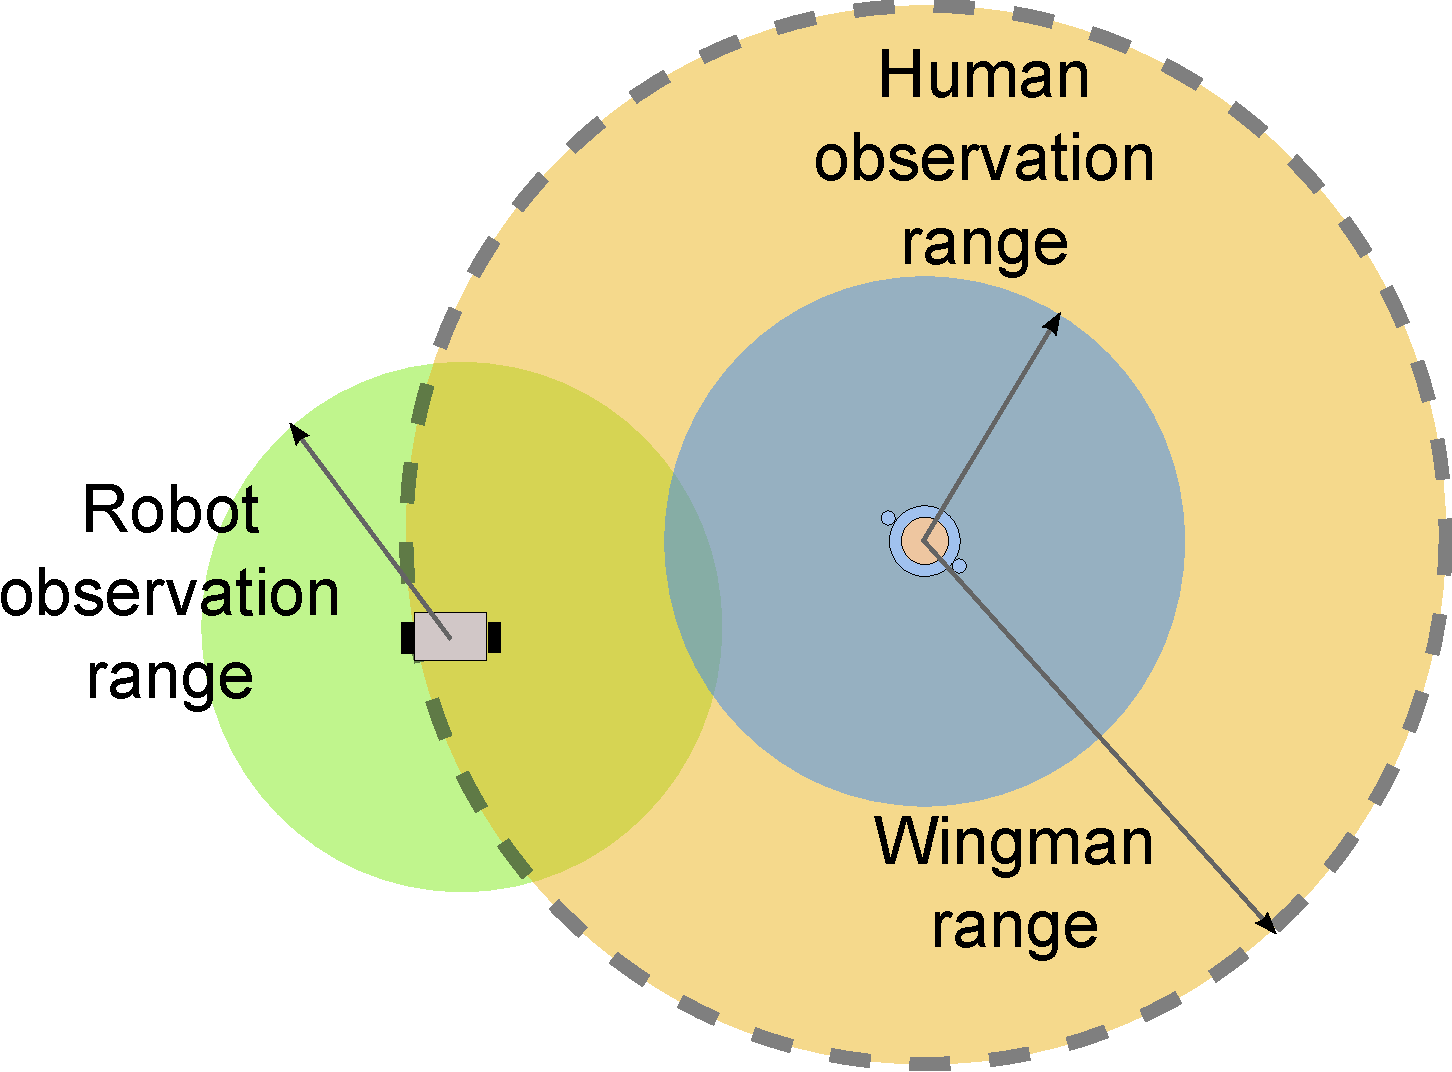
\includegraphics[width = 0.6\textwidth]{./figure/Wingman}
\end{figure}

\end{frame}

\begin{frame}{Labelling}{Robot wingman}

%\begin{minipage}
\begin{columns}
\column{0.25\textwidth}

\column{0.4\textwidth}
\begin{minipage}{\textwidth}
\begin{block}{Gazebo world}
\centering
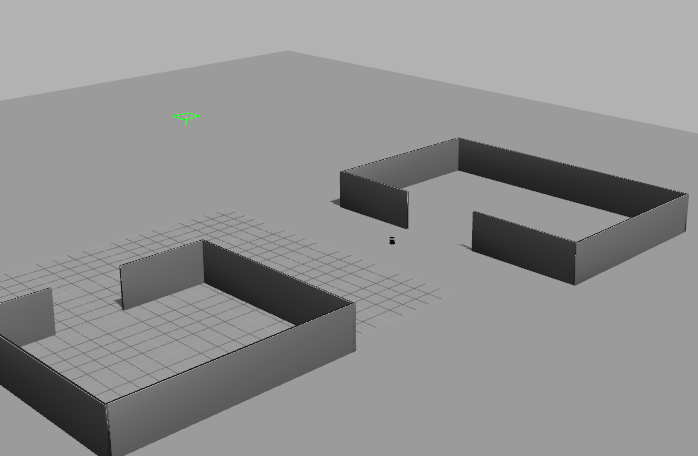
\includegraphics[width = \textwidth]{./figure/simulation/gazebo.png}
\end{block}
\end{minipage}

\column{0.1\textwidth}
\begin{minipage}{\textwidth}
\centering

\includegraphics[width = \textwidth]{./figure/arrow2}
\end{minipage}

\column{0.25\textwidth}
\end{columns}

%\bigskip

\begin{columns}

\column{0.1\textwidth}

\column{0.275\textwidth}
\begin{minipage}{\textwidth}
\begin{block}{Map}
\centering

\includegraphics[width = \textwidth]{./figure/simulation/map.png}
\end{block}
\end{minipage}

\column{0.1\textwidth}
\begin{minipage}{\textwidth}
\centering

\includegraphics[width = \textwidth]{./figure/arrow2}
\end{minipage}

\column{0.275\textwidth}
\begin{minipage}{\textwidth}
\begin{block}{Labeling}
\centering
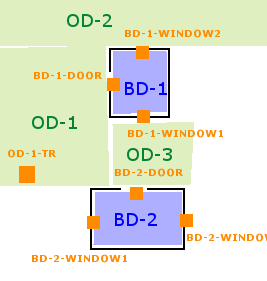
\includegraphics[width = \textwidth]{./figure/simulation/label.png}
\end{block}
\end{minipage}

\column{0.1\textwidth}

\end{columns}
%\end{minipage}

\end{frame}

\begin{frame}{Path planning}{Robot wingman}

\begin{columns}
\column{0.05\textwidth}

\column{0.275\textwidth}
\begin{minipage}{\textwidth}
\begin{block}{Path planning}
\centering
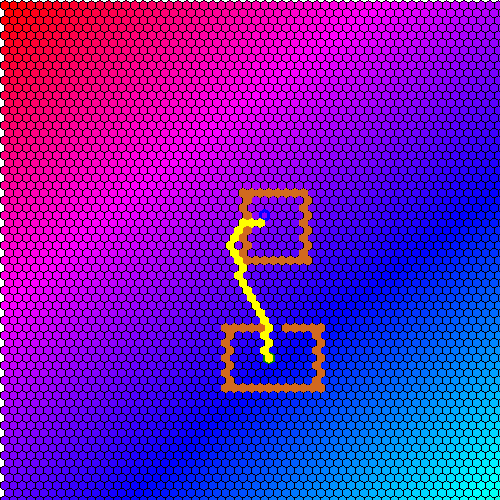
\includegraphics[width = \textwidth]{./figure/simulation/hexamap.png}
\end{block}
\end{minipage}

\column{0.2\textwidth}
\begin{minipage}{\textwidth}
\centering

\includegraphics[width = 0.5\textwidth]{./figure/arrow2}
\end{minipage}

\column{0.275\textwidth}
\begin{minipage}{\textwidth}
\begin{block}{Waypoints}
\centering
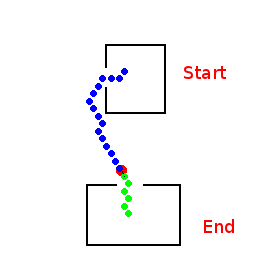
\includegraphics[width = \textwidth]{./figure/simulation/waypoint.png}
\end{block}
\end{minipage}

\column{0.05\textwidth}
\end{columns}

%\bigskip

\begin{columns}
\column{0.25\textwidth}

\column{0.1\textwidth}
\begin{minipage}{\textwidth}
\centering

\includegraphics[width = \textwidth]{./figure/arrow2}
\end{minipage}

\column{0.4\textwidth}
\begin{minipage}{\textwidth}
\begin{block}{Robot execution}
\centering
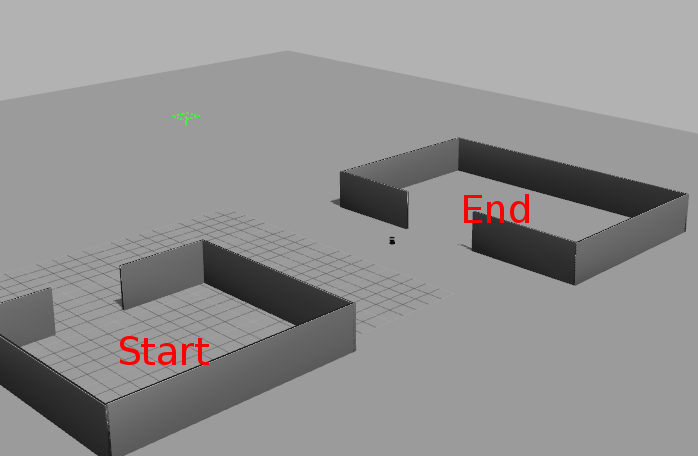
\includegraphics[width = \textwidth]{./figure/simulation/gazebo2.png}
\end{block}
\end{minipage}

\column{0.25\textwidth}

\end{columns}

\end{frame}

\subsection{Results}

\begin{frame}{Metrics}{Results}

\begin{itemize}
\item \textcolor{metric-PR}{\textbf{Problem size}} \\
nodeNum(\dashuline{fully expanding tree}) 
\bigskip
\item \textcolor{metric-NE}{\textbf{Percentage of nodes explored}}
%\textcolor{green}{[efficiency]}
\\
nodeNum(\dashuline{current expanding tree}) / nodeNum(\dashuline{fully expanding tree})
\bigskip
\item \textcolor{metric-OFI}{\textbf{Percentage of optimal at first iteration}}
%\textcolor{red}{[goodness]}
\\
score(\dashuline{first found solution}) / score(\dashuline{optimal solution})
\bigskip
\item \textcolor{metric-IRO}{\textbf{Number of iterations to reach optimal (normalized)}}
%\textcolor{red}{[goodness]}
\\
iterationCount(\dashuline{optimal found}) / iterationCount(\dashuline{finish tree expanding})
\end{itemize}

\end{frame}

\begin{frame}{Metrics}{Results}

\begin{columns}

\column{0.3\textwidth}
\begin{minipage}{\textwidth}
\begin{block}{quality of heuristic}
{\small 
\textcolor{metric-OFI}{Percentage of optimal at first iteration}
}
\end{block}
\end{minipage}

\column{0.7\textwidth}
\begin{figure}
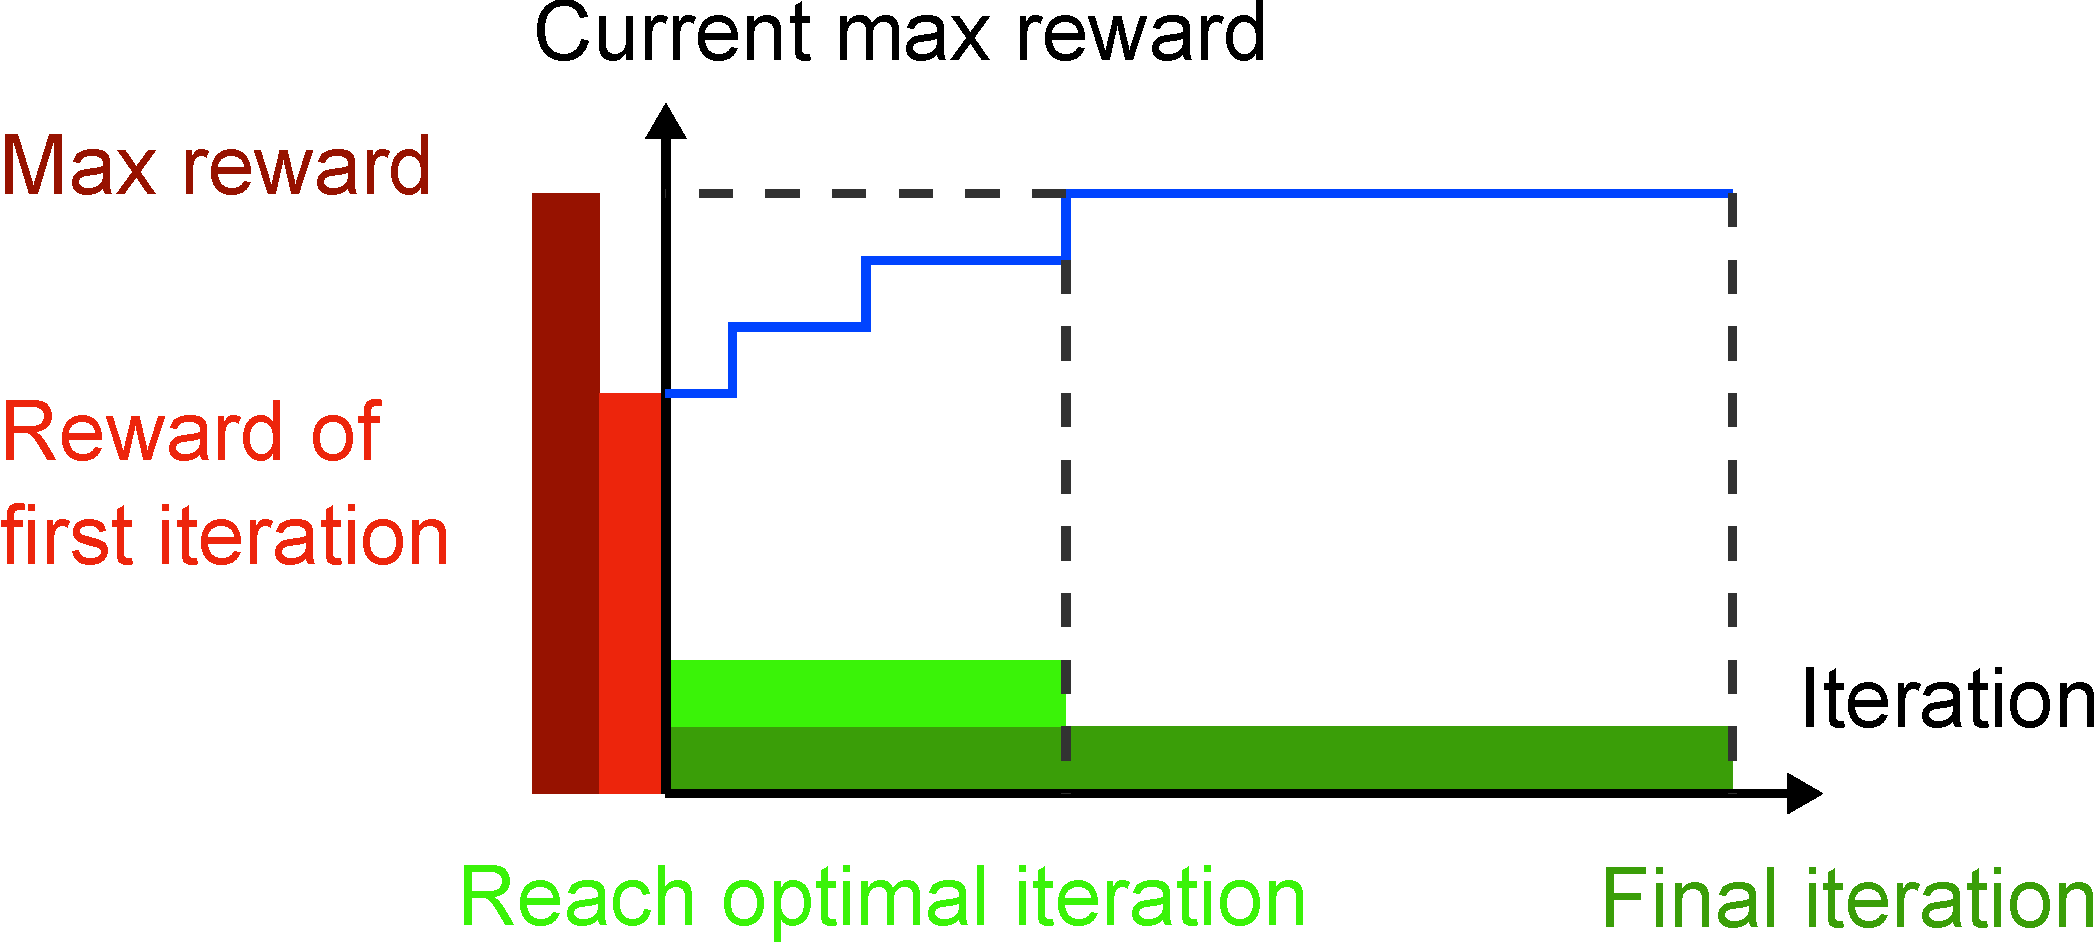
\includegraphics[width=\textwidth]{./figure/metric2}
\end{figure}

\end{columns}

\begin{columns}

\column{0.3\textwidth}

\column{0.7\textwidth}
\begin{center}
\begin{minipage}{0.43\textwidth}
\begin{block}{quality of algorithm}
{\small 
\textcolor{metric-IRO}{Number of iterations to reach optimal (normalized)}
}
\end{block}
\end{minipage}
\end{center}

\end{columns}

\end{frame}

\begin{frame}{Performance}{Results}

\begin{center}
average on the results of 20 runs @ random pattern
\end{center}

\begin{columns}
\column{0.45\textwidth}
\begin{minipage}{\textwidth}
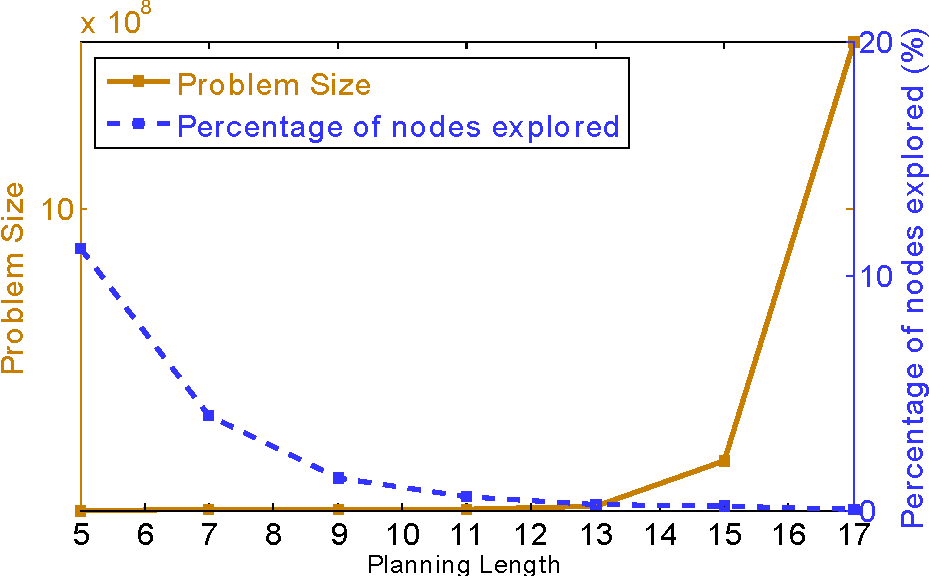
\includegraphics[width=\textwidth]{./figure/T_ProbSize_ExpRatio}
\end{minipage}
\column{0.45\textwidth}
\begin{minipage}{\textwidth}
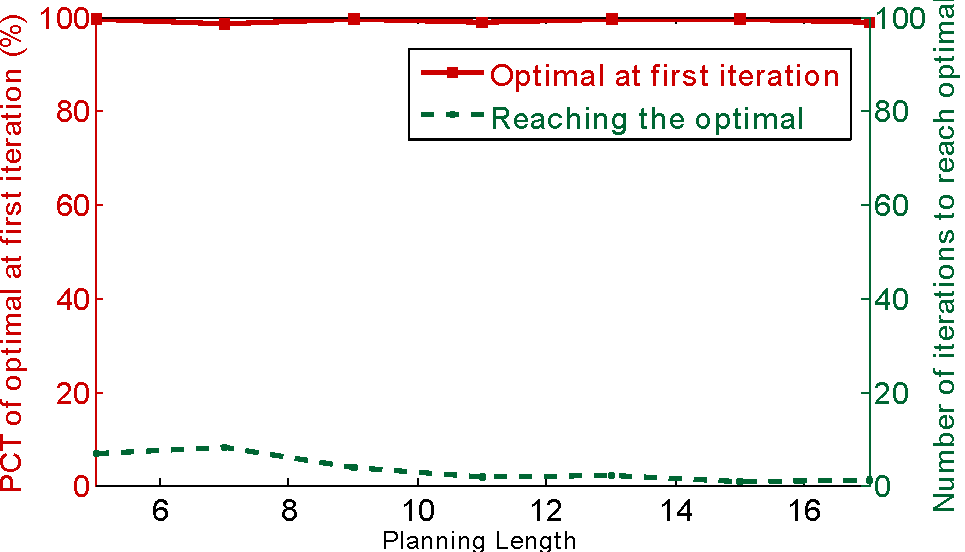
\includegraphics[width=\textwidth]{./figure/T_InitOpt_OptRch}
\end{minipage}
\end{columns}

\begin{columns}
\column{0.5\textwidth}
\begin{center}
{\small 
\textcolor{metric-PR}{Problem size} \\
\textcolor{metric-NE}{Percentage of nodes explored}
}
\end{center}
\column{0.5\textwidth}
\begin{center}
{\small 
\textcolor{metric-OFI}{Percentage of optimal at first iteration} \\
\textcolor{metric-IRO}{Number of iterations to reach optimal (normalized)}
}
\end{center}
\end{columns}

\end{frame}

\begin{frame}{Compare with greedy heuristic}{Performance}

\begin{center}
The quality of the heuristic 
\end{center}

%\begin{columns}
%\column{0.45\textwidth}
%\begin{minipage}{\textwidth}
%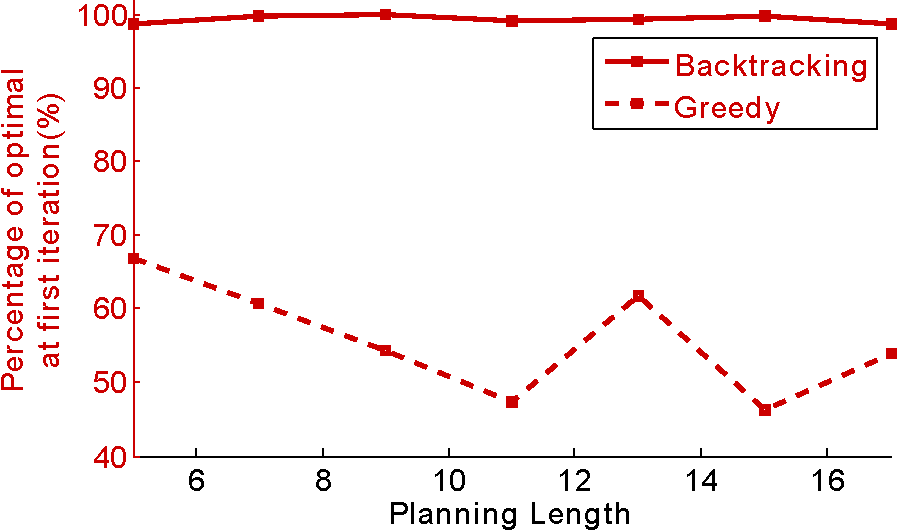
\includegraphics[width=\textwidth]{./figure/compareGreedy}
%\end{minipage}
%\column{0.45\textwidth}
%\begin{minipage}{\textwidth}
%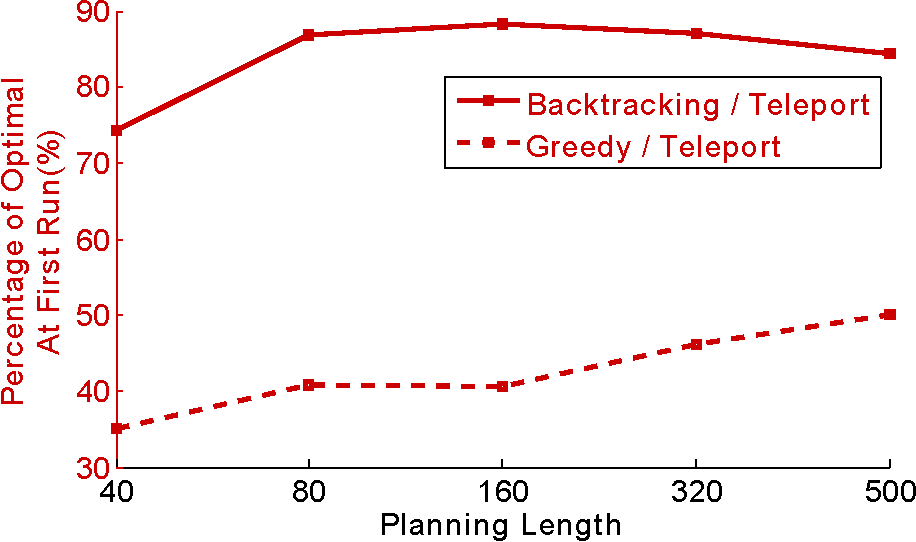
\includegraphics[width=\textwidth]{./figure/largeprob}
%\end{minipage}
%\end{columns}

\begin{figure}
\centering
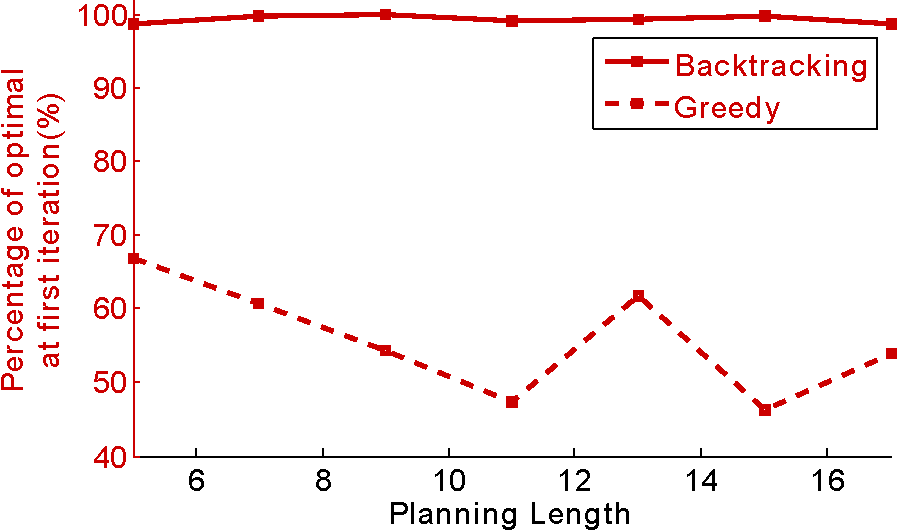
\includegraphics[width=0.6\textwidth]{./figure/compareGreedy}
\end{figure}

\begin{center}
{\small 
\textcolor{metric-OFI}{Percentage of optimal at first iteration}
}
\end{center}

\end{frame}

\begin{frame}{Information pattern difference}{Robustness}

\begin{columns}

\column{0.22\textwidth}
\begin{block}{Uniform}
\begin{center}

\includegraphics[width=0.8\textwidth]{./figure/ENV_UNI}
\end{center}
\end{block}
\column{0.22\textwidth}
\begin{block}{Random}
\begin{center}
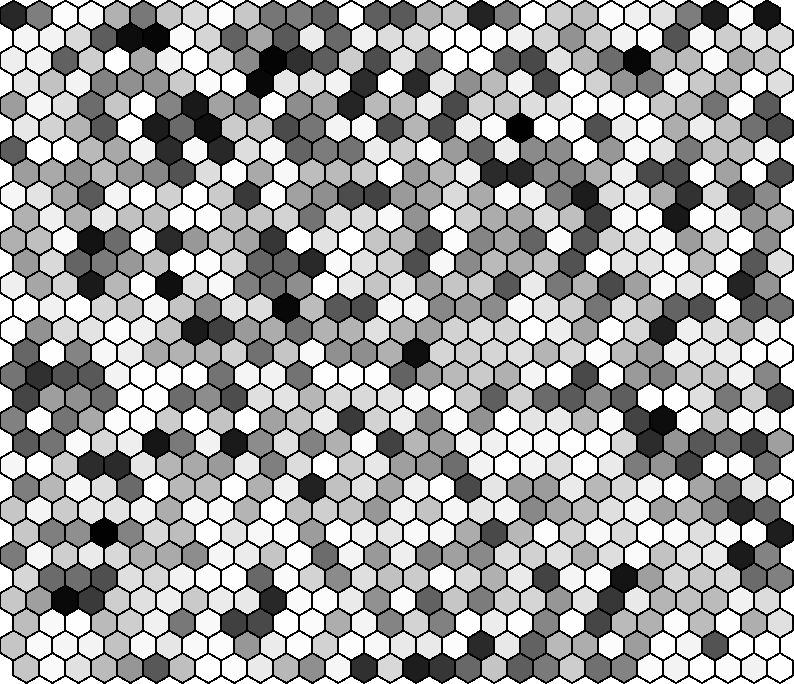
\includegraphics[width=0.8\textwidth]{./figure/ENV_RND}
\end{center}
\end{block}
\column{0.22\textwidth}
\begin{block}{Multi-Modal}
\begin{center}
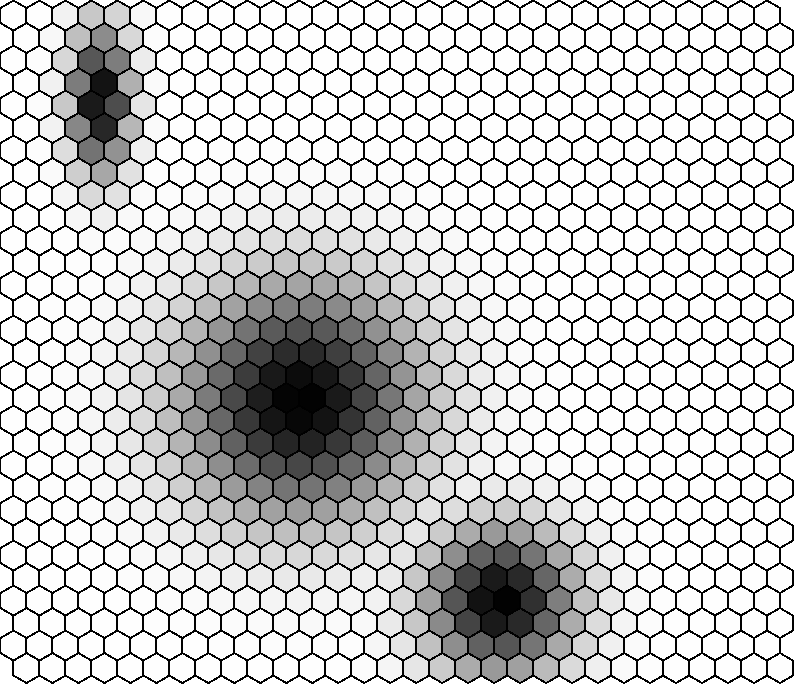
\includegraphics[width=0.8\textwidth]{./figure/ENV_MM}
\end{center}
\end{block}

\end{columns}

\begin{center}
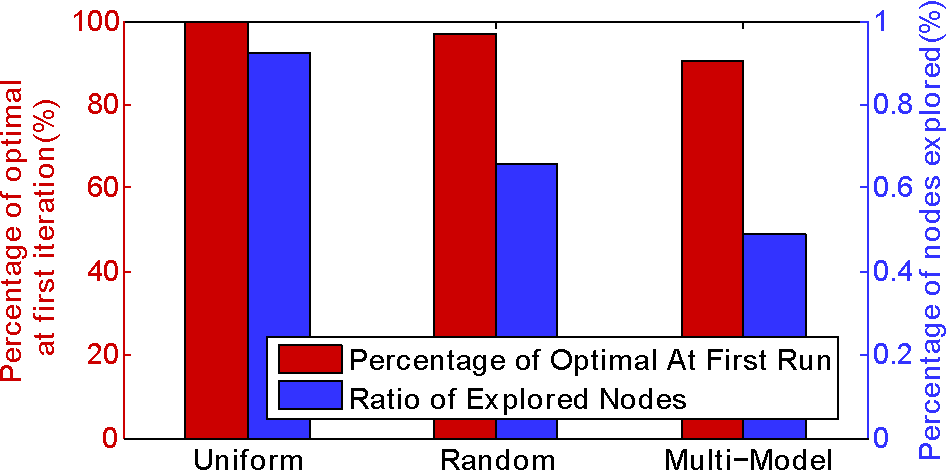
\includegraphics[width=0.6\textwidth]{./figure/EnvPerform}
\end{center}

\begin{columns}
\column{0.5\textwidth}
\begin{center}
{\small
\textcolor{metric-OFI}{Percentage of optimal at first iteration}
}
\end{center}
\column{0.5\textwidth}
\begin{center}
{\small
\textcolor{metric-NE}{Percentage of nodes explored}
}
\end{center}
\end{columns}


\end{frame}

\begin{frame}{Human path difference}{Robustness}

\begin{columns}[T]
\column{.3\linewidth}
\begin{block}{Line}
\begin{minipage}[c][.2\textheight][c]{\linewidth}
\begin{figure}
\centering
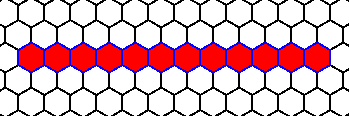
\includegraphics[width = 0.8\textwidth]{./figure/HMP_Line_Small.png}
\end{figure}
\end{minipage}
\end{block}

\column{.3\linewidth}
\begin{block}{Spiral}
\begin{minipage}[c][.2\textheight][c]{\linewidth}
\begin{figure}
\centering
\includegraphics[width = 0.4\textwidth]{./figure/HMP_Spiral_Small.png}
\end{figure}
\end{minipage}
\end{block}

\column{.3\linewidth}
\begin{block}{Lawn mower}
\begin{minipage}[c][.2\textheight][c]{\linewidth}
\begin{figure}
\centering
\includegraphics[width = 0.33\textwidth]{./figure/HMP_LawnMower_Small.png}
\end{figure}
\end{minipage}
\end{block}
\end{columns}

\bigskip

\begin{columns}[T]
\column{.3\linewidth}
\begin{block}{Arc}
\begin{minipage}[c][.2\textheight][c]{\linewidth}
\begin{figure}
\centering
\includegraphics[width = 0.7\textwidth]{./figure/HMP_Arc_Small.png}
\end{figure}
\end{minipage}
\end{block}

\column{.3\linewidth}
\begin{block}{Loitering}
\begin{minipage}[c][.2\textheight][c]{\linewidth}
\begin{figure}
\centering
\includegraphics[width = 0.4\textwidth]{./figure/HMP_Loitering_Small.png}
\end{figure}
\end{minipage}
\end{block}
\end{columns}

\end{frame}

\begin{frame}{Human path difference}{Robustness}

\begin{columns}

\column{0.4\textwidth}
\begin{minipage}{\textwidth}
%\begin{center}
%Problem size
%\end{center}
\begin{figure}
\centering
\includegraphics[width=\textwidth]{./figure/ProbSizeInDiffHMP}
\end{figure}
\begin{center}
{\small
\textcolor{metric-PR}{Problem size}
}
\end{center}
\end{minipage}

\column{0.4\textwidth}
\begin{minipage}{\textwidth}
%\begin{center}
%Ratio of explored nodes
%\end{center}
\begin{figure}
\centering
\includegraphics[width=\textwidth]{./figure/ExpRatioInDiffHMP}
\end{figure}
\end{minipage}
\begin{center}
{\small
\textcolor{metric-NE}{Percentage of nodes explored}
}
\end{center}
\end{columns}

\bigskip

\begin{columns}
\column{0.6\textwidth}
\begin{minipage}{\textwidth}
%\begin{center}
%Percentage of optimal at first run
%\end{center}
\begin{figure}
\centering
\includegraphics[width=0.7\textwidth]{./figure/InitOptInDiffHMP}
\end{figure}
\end{minipage}
\begin{center}
{\small
\textcolor{metric-OFI}{Percentage of optimal at first iteration}}
\end{center}
\end{columns}

\end{frame}

\section{Summary}
\label{sec:summary}

In this paper, we use a human path to form a path constraint and seek to maximize the information gathered by a robot gathered in a search task.
The resulting information maximization path planning is identified as a constrained submodular orienteering problem on a multi-partite graph.
We present an anytime algorithm that used a planning heuristic based on backtracking to efficiently find a high quality path.
We use a node freeze process to avoid an exhaustive search, yet we prove that this process always preserves the ability of the algorithm to find an optimal solution.
We have also shown empirically that this approach substantially reduces the complexity of the resulting search.

% All of the following is optional and typically not needed. 

\end{document}


